%%
\documentclass[12pt,a4paper,english,greek,twoside]{ece-thesis}

\usepackage{graphicx}
\usepackage{epstopdf}
\usepackage{indentfirst}
\usepackage{verbatim}
\usepackage{amsmath}
\usepackage{amsthm}
\usepackage{amssymb}
\usepackage{latexsym}
\bibliographystyle{plain}
\usepackage{hyphenat}
\usepackage{makeidx}
\usepackage{dirtytalk}
\addto\captionsgreek{%
  \renewcommand{\indexname}{Ευρετήριο όρων}%
}
\makeindex

% 1.5 spacing
\renewcommand{\baselinestretch}{1.2}

% latin text (and greek text)
\newcommand{\tl}[1]{\textlatin{#1}}
\newcommand{\tg}[1]{\textgreek{#1}}

% typeset short english phrases
\newcommand{\en}[1]{\foreignlanguage{english}{#1}}

% typeset source code
\newcommand{\src}[1]{{\tt\en{#1}}}

% typeset a backslash
\newcommand{\bkslash}{\en{\symbol{92}}}

\newtheorem{definition}{Ορισμός}
\newtheorem{proposition}{Πρόταση}
\newtheorem{theorem}{Θεώρημα}
\newtheorem{corollary}{Συμπέρασμα}
\newtheorem{lemma}{Λήμμα}
\newtheorem{example}{Παράδειγμα}
\newtheorem{remark}{Σημείωση}
\newtheorem{notation}{Συμβολισμός}
\newtheorem{law}{Νόμος}
\renewcommand{\thedefinition}{\arabic{chapter}.\arabic{definition}}
\renewcommand{\theproposition}{\arabic{chapter}.\arabic{proposition}}
\renewcommand{\thetheorem}{\arabic{chapter}.\arabic{theorem}}
\renewcommand{\thecorollary}{\arabic{chapter}.\arabic{corollary}}
\renewcommand{\thelemma}{\arabic{chapter}.\arabic{lemma}}
\renewcommand{\theexample}{\arabic{chapter}.\arabic{example}}
\newcommand{\set}[1]{\left\{#1\right\}}
\newcommand{\To}{\Longrightarrow}
\newcommand{\xml}{\en{XML}}

\selectlanguage{greek}

\hyphenation{ο-ποί-α}

%%%%%%%%%%%%%%%%%%%%%%%%%%%%%%%%%%%%%%%%%%%%%%%%%%%%%
%% THESIS INFO 
%%
%
% Τίτλος Πτυχιακής Εργασίας
	\title{Πρόβλεψη Συνδέσμων σε Γράφους με Χρήση Tεχνικών Μηχανικής Μάθησης}
% "του" ή "της", ανάλογα με το φύλο του σπουδαστή
	\edef\toutis{του}
% Ονοματεπώνυμο σπουδαστή (ΚΕΦΑΛΑΙΑ, γενική πτώση)
	\edef\authorNameCapital{ΧΑΜΕΖΟΠΟΥΛΟΥ ΣΑΒΒΑ}
% Ονοματεπώνυμο σπουδαστή (πεζά, ονομαστική πτώση)
	\author{Χαμεζόπουλος Σάββας}
% Ονοματεπώνυμο Επιβλέποντα Καθηγητή
	\supervisor{Παπαλάμπρου Κωνσταντίνος}
    \edef\supervisorTitle{Λέκτορας}
% "Επιβλέπων" ή "Επιβλέπουσα", ανάλογα με το φύλο του Επιβλέποντα Καθηγητή
	\edef\supervisorMaleFemale{Επιβλέπων}
% Τόπος, μήνας και έτος
	\edef\thesisPlaceDate{Θεσσαλονίκη, Ιούλιος 2020}
% Ημερομηνία Εξέτασης
	\edef\examinationDate{10η Ιουλίου 2020}
% Έτος Copyright
	\edef\copyrightYear{2020}
% Ονοματεπώνυμο 1ου εξεταστή
	\epitropiF{Πιτσούλης Λεωνίδας}
% Τίτλος 1ου εξεταστή
	\edef\epitropiFTitle{Αναπληρωτής Καθηγητής}
% Ονοματεπώνυμο 2ου εξεταστή
	\epitropiS{Μπίσκας Παντελής}
% τίτλος 2ου εξεταστή
	\edef\epitropiSTitle{Αναπληρωτής Καθηγητής}
%%%%%%%%%%%%%%%%%%%%%%%%%%%%%%%%%%%%%%%%%%%%%%%%%%%%%


\begin{document}
\selectlanguage{greek}
\maketitle

\frontmatter
% Περίληψη
	\begin{abstract}

Η ανάπτυξη της επιστημονικής μελέτης της  εξέλιξης των δικτύων έχει φέρει μια νέα εποχή στην επίλυση διαφόρων πρακτικών προβλημάτων. Παράλληλα, οι τεχνικές μηχανικής μάθησης, αλλα και γενικότερα της τεχνητής νοημοσύνης,
επιταχύνουν και βελτιώνουν τον τρόπο που η πληροφορία επεξεργάζεται, διευκολύνοντας και επιταχύνοντας
σημαντικά την επίλυση υπερβολικά χρονοβόρων ή και άλυτων μέχρι σήμερα προβλημάτων. Η τελευταία καινοτομία
στο χώρο της θεωρίας δικτύων και της ανάλυσης φαινομένων με χρήση τεχνητής νοημοσύνης υποστηρίζει το συνδυασμό των 
δύο, δηλαδή επίλυσης προβλημάτων δικτύων με χρήση τεχνικών μηχανικής μάθησης. Οι εφαρμογές της παραπάνω προσέγγισης βρίσκονται
σε πολυάριθμους τομείς.  Στα πλαίσια της εργασίας αυτής επιλέχθηκαν δύο περιπτώσεις προς ανάλυση από διαφορετικούς τομείς. Η πρώτη ασχολείται με ένα δίκτυο αναφορών σε  επιστημονικές δημοσιεύσεις ενώ η δεύτερη με ένα δίκτυο που αφορά την εμπιστοσύνη μεταξύ χρηστών σε πλατφόρμα
συναλλαγών κρυπτονομισμάτων. Σκοπός της εργασίας, είναι να προβλεφθούν, στην πρώτη περίπτωση, οι νέες αναφορές μεταξύ των
επιστημονικών εργασιών στο δοθέν δίκτυο και, στη δεύτερη περίπτωση,  η κίνηση της αγοράς πάνω σε μία από τις γνωστότερες πλατφόρμες συναλλαγών
κρυπτονομισμάτων. Για το σκοπό αυτό χρησιμοποιούμε δεδομένα γράφων σε συνδυασμό με μια πληθώρα τεχνικών 
μηχανικής μάθησης, με ένα νέο συνδυαστικό τρόπο, στην αναζήτηση της αποδοτικότερης λύσης με σκοπό την
ανάπτυξη ενός ολοκληρωμένου συστήματος πρόβλεψης συνδέσεων σε γράφους.
 
   \begin{keywords}

   Πρόβλεψη Συνδέσμων, Λογιστική Παλινδρόμιση, Βεβαρημένα Δίκτυα, Αναπαράσταση Κόμβων, 
   \tl{Node2Vec, GraphSAGE, CTDNE} 
   \end{keywords}
\end{abstract}



\begin{abstracteng}
\tl{The recent advances on the scientific examination of the evolvement of  networks has improved dramatically the solution techniques regarding various practical problems. At the same 
time, machine learning, a subcategory of artificial intelligence algorithms and techniques, has been used
more and more in solving complex and previously time-consuming and/or unsolvable tasks. The latest trend
in the field of network theory and machine learning has the two combined, in order to achieve 
unprecedented results. The applications of the aforementioned approach span many different areas. In this thesis, two cases from different areas are examined. The first one  concerns a citation network of scientific publications while the second one concerns a trust network among users of a cryptocurrency platform.
The main aim of this work, in the first case, is to predict future citations in the given network of publications  and, in the second case, to predict the future state of  a network consisting of users of
a well-known cryptocurrency platform. To achieve that, these cases are viewed as link prediction problems and we utilize graph data available for these networks and use various machine learning techniques in order to provide the most efficient solution.}

   \begin{keywordseng}
       \noindent
   \tl{ Link Prediction, Logistic Regression, Weighted Networks, Node Embedding, Node2Vec, GraphSAGE, CTDNE}
   \end{keywordseng}

\end{abstracteng}
% Αφιέρωση
	\thesisDedication{στους γονείς και τον αδελφό μου}
% Ευχαριστίες
	\begin{acknowledgements}
Θα ήθελα καταρχήν να ευχαριστήσω τον Λέκτορα κ. Κωνσταντίνο Παπαλάμπρου 
για την επίβλεψη αυτής της διπλωματικής εργασίας και για την
εξαιρετική συνεργασία που μου πρόσφερε καθ' όλη τη διάρκεια αυτής. 
Επίσης θα ήθελα να ευχαριστήσω τους γονείς
μου, Κωνσταντίνο και Μαριάννα, καθώς και τον αδερφό μου Ελευθέριο,
για την καθοδήγηση και την ηθική συμπαράσταση που μου
προσέφεραν όλα αυτά τα χρόνια.
\end{acknowledgements}
% Πίνακας Περιεχομένων
	\tableofcontents
% Κατάλογος Σχημάτων
	\listoffigures
% Κατάλογος Πινάκων
	\listoftables

%%%%%%%%%%%%%%%%%%%%%%%%%%%%%%%%%%%%%%%%%%%%%%%%%%%%%
%% INCLUDE YOUR CHAPTERS/SECTIONS HERE
%%
\mainmatter
% Εισαγωγή
    \chapter{Εισαγωγή}

Η έννοια των δικτύων υπήρχε από πολύ παλιά τόσο στη ζωή και στη φύση, όσο και στην κοινωνία των ανθρώπων.
Από τις συνδέσεις των ατόμων που σχηματίζουν μόρια, μέχρι τις πόλεις και το ίδιο το διαδίκτυο, παντού
τριγύρω μας μπορούμε να διακρίνουμε συμπλέγματα οντοτήτων που αλληλοεπιδρούν αναμεταξύ τους. Με την 
ανάπτυξη των υπολογιστών και των υπολογιστικών συστημάτων, καθώς και με την πρόοδο των μαθηματικών
έγινε δυνατή η ανάλυση και η εξαγωγή πληροφορίας και γνώσης που κρύβουν τα δίκτυα μέσα τους. Παράλληλα,
η ραγδαία ανάπτυξη της τεχνητής νοημοσύνης και ιδιαίτερα των τεχνικών μηχανικής μάθησης, έφερε μια νέα
εποχή στην ανάλυση και επίλυση μιας πληθώρας προβλημάτων, καθιστώντας επιλύσιμα πολύ περίπλοκα ζητήματα
με υψηλή ακρίβεια και σε σχετικά μικρό χρόνο.

Πολλά προβλήματα της καθημερινής ζωής είναι δυνατόν να λυθούν με χρήση θεωρίας δικτύων και χρήση 
υπολογιστικών συστημάτων. Μερικά από τα πιο γνωστά είναι:

\begin{itemize}
    \item Ταξινόμηση Κόμβων
    \item Ομαδοποίηση Κόμβων
    \item Πρόβλεψη συνδέσεων
    \item Οπτικοποίηση Δικτύου
    \item και άλλα (κ.α.)
\end{itemize}

Στην εργασία αυτή θα ασχοληθούμε με το πρόβλημα της πρόβλεψης συνδέσεων σε  γράφους, οι οποίοι αποτελούν μια μορφή μοντελοποίησης
 των δικτύων. Το πρόβλημα  την πρόβλεψης συνδέσεων συναντάται συχνότατα τόσο στην καθημερινή ζωή,
όσο και σε πιο εξειδικευμένες περιπτώσεις τόσο στην κοινωνία όσο και στην οικονομία και τη φύση.
Ένα πολύ διαισθητικά κατανοητό παράδειγμα βρίσκεται στα μέσα κοινωνικής δικτύωσης \cite{al2011survey}. 
Οι εταιρίες πίσω 
από τις εν λόγω πλατφόρμες, προκειμένου να διατηρούν τους χρήστες ενεργούς, καλούνται να τους
προτείνουν να συνδεθούν με άτομα που πιθανόν να γνωρίζουν, να τους προτείνουν υλικό και σελίδες που
πιθανόν τους ενδιαφέρουν κ.α. Από την άλλη, στις πλατφόρμες διαδικτυακών αγορών, προτείνονται στους
χρήστες προϊόντα προς πώληση που πιθανόν τους ενδιαφέρουν, βάσει του δικού τους ιστορικού  ή  άλλων
χρηστών.
Ακόμα και σε θέματα ασφάλειας έχουν υλοποιηθεί εργαλεία με χρήση της πρόβλεψης συνδέσεων 
\cite{berlusconi2016link}. Τέλος, μια εφαρμογή του προβλήματος της πρόβλεψης συνδέσεων στην οικονομία
και πιο συγκεκριμένα στο χρηματιστήριο είναι η πρόβλεψη της κίνησης της αγοράς, με την έννοια της
πρόβλεψης των τασεων της αγοράς και της αυξομοίωσης της ζήτησης των μετοχών 
\cite{stockpred}, \cite{Souza_2019}.

Συγκεκριμένα, στην εργασία αυτή θα ασχοληθούμε με δύο εφαρμογές του προβλήματος της πρόβλεψης συνδέσμων.
Αρχικά, θα προσπαθήσουμε να προβλέψουμε τις συνεργασίες μεταξύ επιστημόνων στο μέλλον, χρησιμοποιώντας
δεδομένα αναφορών από έναν επιστήμονα σε κάποιον άλλον στις δημοσιεύσεις τους. Επιπλέον, θα 
προσπαθήσουμε να προβλέψουμε την κίνηση της αγοράς του κρυπτονομίσματος \en{Bitcoin} μέσω της 
πλατφόρμας \en{OTC}. Για τον σκοπό αυτό, θα χρησιμοποιήσουμε δεδομένα βαθμολόγησης μεταξύ των χρηστών,
και θεωρούμε πως ένας χρήστης με υψηλή βαθμολογία θα εκτελεί περισσότερες συναλλαγές στο μέλλον, 
αφού οι υπόλοιποι θα τον προτιμούν, ενώ ένας χρήστης με χαμηλότερη βαθμολογία σταδιακά θα πάψει
να συναλλάσσεται αφού δε θα υπάρχουν ενδιαφερόμενοι να αγοράσουν από ή να πουλήσουν σε αυτόν.

\section{Διατύπωση του προβλήματος} \label{problem_statement}

Το πρόβλημα που θα αναλυθεί στην εργασία αυτή διατυπώνεται ως εξής:
Δεδομένου ενός γράφου που μεταβάλλεται χρονικά, θα γίνει μια προσπάθεια πρόβλεψης των μελλοντικών συνδέσεων. Αυτή η δήλωση 
ισοδυναμεί με τη σκέψη πως αν έχουμε διαθέσιμη μια εικόνα του δικτύου κάποια στιγμή στο παρελθόν, 
τότε θα προσπαθήσουμε να διατυπώσουμε την εικόνα του γράφου αυτού στο παρόν, προβλέποντας τις νέες 
συνδέσεις. Άρα θα πρέπει να κατασκευαστεί μια εικόνα του γράφου όπως αυτή ήταν στο παρελθόν. Χωρίς
βλάβη της γενικότητας, για το σκοπό αυτό κάνουμε την εξής θεώρηση: Στο γράφο με την πάροδο του χρόνο
δεν διαγράφονται συνδέσεις (ακμές) παρά μόνο δημιουργούνται νέες. Επομένως σε μια παρελθοντική στιγμή
απλώς θα υπήρχαν λιγότερες συνδέσεις, και προφανώς θα φτάσουμε στην εικόνα αυτή του γράφου διαγράφοντας
κάποιες ακμές με τυχαίο τρόπο.

Ξεκινώντας λοιπόν με μια εικόνα του γράφου στο παρελθόν, όπως αναφέρθηκε, με χρήση τεχνικών μηχανικής
μάθησης θα επιχειρήσουμε να προβλέψουμε, ή αλλιώς να ανακαλύψουμε τις νέες συνδέσεις που θα προκύψουν
μέχρι το παρόν. Για την επίτευξη του σκοπού αυτού, θα ακολουθηθεί η εξής λογική: Σκοπός είναι να 
προβλεφθούν νέες συνδέσεις, ή διαφορετικά, να προβλεφθεί ορθά αν μια σύνδεση (ακμή) είναι αληθής ή 
όχι. Συνεπώς το ζήτημα ανάγεται σε ένα πρόβλημα δυαδικής ταξινόμησης, και απαντάται το ερώτημα αν μια
ακμή υπάρχει (1) ή δεν υπάρχει (0). Οπότε θα χρησιμοποιηθεί ένας δυαδικός ταξινομητής. Για τη 
λειτουργία του ταξινομητή θα πρέπει να αναπαρασταθούν τα δεδομένα σε κατάλληλη μορφή, αφού η αρχική
μορφή του γράφου δεν είναι συμβατή με τέτοια συστήματα. Για την επίτευξη του σκοπού αυτού θα 
χρησιμοποιηθούν διάφορες τεχνικές αναπαράστασης γράφων. Κλείνοντας, να αναφερθεί ότι στην αναπαράσταση των δεδομένων 
χρησιμοποιούνται τεχνικές βαθειάς μάθησης ενώ όσον αφορά τους ταξινομητές χρησιμοποιούνται τεχνικές επιβλεπόμενης μάθησης.

\section{Δομή της εργασίας}

Η εργασία χωρίζεται σε τρείς ενότητες. Αρχικά θα δοθούν κάποια βασικά στοιχεία θεωρίας γράφων, ανάλυσης
δικτύων και κάποια στοιχεία σχετικά με τη μηχανική μάθηση. Θα παρουσιαστεί δηλαδή σύντομα όλο το θεωρητικό υπόβαθρο
πάνω στο οποίο βασίστηκε η εργασία αυτή. Επίσης, θα αναλυθούν σε βάθος οι τεχνικές αναπαράστασης 
γράφων. Στο δεύτερο σκέλος θα παρουσιαστεί η μεθοδολογία που ακολουθήθηκε καθώς και η δομή των πειραμάτων
ώστε να μπορεί ο αναγνώστης να αναπαράξει επακριβώς τα πειράματα,
ενώ στο τρίτο σκέλος θα δοθούν οι ακριβείς συνθήκες κάτω από τις οποίες πραγματοποιήθηκαν τα πειράματα,
καθώς και τα αποτελέσματα αυτών. Τέλος, θα δοθούν συγκεκριμένα συμπεράσματα και θα προταθούν 
ενδεχόμενες μελλοντικές επεκτάσεις που μπορούν να εξεταστούν.	
% Κεφάλαια
    \chapter{\selectlanguage{greek}Θεωρητικό Υπόβαθρο}

Στο κεφάλαιο αυτό παρουσιάζονται αρχικά κάποια στοιχεία της θεωρίας γραφημάτων. Έπειτα δίνονται 
κάποια βασικά στοιχεία σχετικά με τη μηχανική μαθηση και ειδικότερα για τα παρακλάδια αυτής
που χρησιμοποιήθηκαν.

\section{Βασικά στοιχεία θεωρίας γραφημάτων}
\subsection{Βασικοί ορισμοί}

Στην Θεωρία  Γραφημάτων ή Γράφων (\en{Graph Theory}), ένας γράφος \(G = (V,E)\)  είναι δομή δεδομένων που
αποτελείται από ένα σύνολο κόμβων \(V\)(\en{nodes}) και ακμών \(E\) (\en{edges}), που 
συνδέουν τους κόμβους μεταξύ τους \cite{Diestel} \cite{barabasi}. Συνήθως ένας γράφος
αναπαρίσταται ως τελείες που συμβολίζουν τους κόμβους και γραμμές μεταξύ των τελειών που
συμβολίζουν τις ακμές. Η σειρά που αναπαριστώνται οι γραμμές και οι τελείες δεν έχει σημασία,
αφού οι γράφοι διατηρούν την πληροφορία τους στον τρόπο με τον οποίο είναι συνδεδεμένοι οι 
κόμβοι μεταξύ τους.

\begin{figure}[!ht] \centering
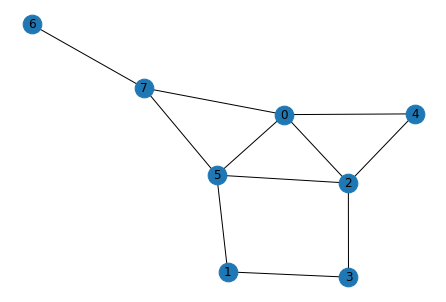
\includegraphics[scale = 0.5]{static/figures/graph_example.png} 
\caption{Παράδειγμα γράφου}
\label{figure1.1}
\end{figure}

Οι γράφοι αποτελούν μια μη-ευκλείδια δομή δεδομένων, που σημαίνει ότι διαφέρουν από
τις παραδοσιακές δομές δεδομένων δύο διαστάσεων, όπως οι εικόνες, ο ήχος και το κείμενο. Οι
κόμβοι αποτελούν οντότητες που συγκρατούν την πληροφορία για κάποιο στοιχείο, ενώ οι ακμές
αντιπροσωπεύουν τη σύνδεση μεταξύ των κόμβων, και μπορούν και αυτές να περιέχουν κάποια
πληροφορία για τη σύνδεση αυτή. Τέλος, οι γράφοι μπορούν να έχουν κάποια χαρακτηριστικά που
ρυθμίζουν τις ενέργειες και την ανάλυση που μπορούμε να εκτελέσουμε πάνω σε αυτούς.

Οι κόμβοι και οι ακμές μπορούν να αποτελούνται από διάφορα στοιχεία:
\begin{itemize}
    \item Είδος (\en{Type})
    \item Ετικέτες (\en{Labels})
    \item Χαρακτηριστικά (\en{Features} (μετάφραση (μτφ.) Γνωρίσματα)/\en{Attributes} (μτφ. Χαρακτηριστικά)
\end{itemize}

Το είδος ενός κόμβου αντιπροσωπεύει την κατηγορία στην οποία εμπίπτει (π.χ. αν αντιπροσωπεύει
άνθρωπο ή κάποιο ζώο). Οι ετικέτες και τα χαρακτηριστικά αποτελούν 2 διαφορετικά στοιχεία,
τα οποία μπορούν να γίνουν διαισθητικά αντιληπτά με το εξής παράδειγμα: εάν ένας κόμβος
συμβολίζει έναν άνθρωπο, τότε η ετικέτα του κόμβου είναι το όνομά του, και τα χαρακτηριστικά
του είναι τα γνωρίσματα που χαρακτηρίζουν το άτομο αυτό (ηλικία, φύλο, εκπαίδευση, κ.λπ.).
Συνήθως στα υπολογιστικά συστήματα για ευκολία ο κάθε κόμβος έχει το δικό του αριθμό
ταυτοποίησης (\en{id}).

Οι ακμές μπορούν να έχουν και αυτές χαρακτηριστικά και ετικέτες (βάρη). Να σημειωθεί εδώ πως
οι ετικέτες και τα χαρακτηριστικά δεν είναι απαραίτητα δεδομένα σε αριθμητική μορφή, αλλά
μπορούν να έχουν και τη μορφή κειμένου.

\subsection{Είδη γράφων} \label{Είδη γράφων}

Στα πλαίσια της παρούσας εργασίας, ένας γράφος \(G\) αποτελείται από μία συνάρτηση χαρτογράφησης ειδών κόμβου \(f_u: V 
\rightarrow T^u\) και αντίστοιχα μια συνάρτηση χαρτογράφησης τύπων ακμών \(F_e: E \rightarrow
T^e\), όπου \(T_u\) και \(T_e\) το σύνολο των ειδών κόμβων και ακμών αντίστοιχα. 

Με βάση τα παραπάνω, οι γράφοι χωρίζονται σε διάφορες κατηγορίες, ανάλογα με το είδος των ακμών και τον κόμβων που τους απαρτίζουν:
\begin{itemize}
    \item \textbf{Ομογενείς}, όταν \(|T^u| = |T^e| = 1\), δηλαδή όλοι ο κόμβοι και οι ακμές 
    είναι ενός τύπου
    \item \textbf{Ετερογενείς}, όταν \(|T^u|>1\) ή/και \(|T^e|>1\), δηλαδή οι κόμβοι ή/και 
    οι ακμές είναι διαφόρων τύπων.
\end{itemize}

Ακόμα, οι γράφοι μπορούν να χαρακτηριστούν ανάλογα με το είδος των ακμών:
\begin{itemize}
    \item \textbf{Μη-κατευθυνόμενοι} (\en{Undirected}), όταν η σύνδεση 2 κόμβων είναι
    αμφίδορμη, δηλαδή μπορεί κανείς να μετακινηθεί από τον κόμβο \(u_a\) στον κόμβο \(u_b\)
    και αντίστροφα μέσω της ίδιας ακμής (\(u_a \leftrightarrow u_b\))
    \item \textbf{Κατευθυνόμενοι} (\en{Directed}), όταν η σύνδεση είναι από τον κόμβο \(u_a\)
    στον κόμβο \(u_b\) προϋποθέτει ακμή αυστηρά από τον κόμβο \(u_a\) προς τον κόμβο \(u_b\)
    (\(u_a \rightarrow u_b\))
\end{itemize}

Επίσης οι γράφοι μπορούν να είναι:
\begin{itemize}
    \item \textbf{Στατικοί}, όταν οι κόμβοι και οι ακμές δεν αλλάζουν 
    π.χ. με την πάροδο του χρόνου 
    \item \textbf{Δυναμικοί}, όταν οι κόμβοι και οι ακμές μπορούν να αλλάξουν, 
    να μετακινηθούν κλπ.
\end{itemize}

Τέλος, ένα \emph{μονοπάτι (\en{path)}} σε ένα γράφο μπορεί να οριστεί ως εξής
\cite{Diestel}: \(P = (V,E)\) όπου \(V =\{x_0,x_1,\cdots,x_k\}\) και
\(E = \{(x_0,x_1),(x_1,x_2),\cdots,(x_{k-1},x_k)\}\), όπου \(V \subseteq V_G\) και \(E 
\subseteq E_G\). Ένας \emph{περίπατος} (\en{walk}) μπορεί να ειδωθεί σαν ένα μονοπάτι  στο οποίο κορυφές ή/και ακμές μπορουν να επαναληφθούν. \emph{Μήκος μονοπατιού/περιπάτου} είναι ο αριθμός των ακμών που περιέχει το μονοπάτι ή ο περίπατος. 

\section{Επιστήμη δικτύων}

Η επιστήμη δικτύων και η θεωρία γράφων είναι δύο βαθιά συσχετιζόμενα επιστημονικά πεδία,
τα οποία ωστόσο έχουν κάποιες διαφορές. Η θεωρία γράφων ασχολείται με τη μαθηματική ανάλυση και παρέχει ένα πλήθος αλγορίθμων
που μπορούν να εφαρμοστούν σε όλους τους γράφους, ανεξαρτήτως του προβλήματος που 
αντιπροσωπεύουν. Η επιστήμη δικτύων εστιάζει σε προβλήματα που βρίσκονται στον πραγματικό
κόσμο. Ο γράφος μετονομάζεται σε δίκτυο, και αναλύονται δίκτυα μεταφορών, κοινωνικά δίκτυα
κ.λπ. Η επιστήμη δικτύων  αναπτύχθηκε παράλληλα  με την των υπολογιστικών συστημάτων.

\subsection{Μετρικές ομοιότητας}

Στην επιστήμη δικτύων μελετάται η δομή και τα χαρακτηριστικά ενός δικτύου με σκοπό την 
εξαγωγή πληροφορίας και συμπερασμάτων για την επίλυση ενός προβλήματος. Για το σκοπό αυτό
έχουν αναπτυχθεί μετρικές ομοιότητας οι οποίες ποσοτικοποιούν την ομοιότητα μεταξύ των 
κόμβων. Αυτή η ανάλυση είναι χρήσιμη διότι σε πολλά προβλήματα στην επιστήμη δικτύων,
σημαντικό μέρος της λύσης αποτελεί η εύρεση ````γειτονιών'''', δηλαδή ομάδων κόμβων με κοινά
χαρακτηριστικά και γειτονικούς κόμβους, ή η εύρεση ````όμοιων'''' κόμβων σύμφωνα με κάποιες μετρικές.
Στη συνέχεια θα παρουσιαστούν ορισμένες από αυτές, οι οποίες είναι σχεδιασμένες έτσι ώστε
με δεδομένους 2 κόμβους, μια μετρική να δίνει υψηλότερη τιμή αν οι 2 κόμβοι είναι ````όμοιοι''''.

\subsubsection{Απόσταση}

Η Απόσταση (\en{Graph Distance}) εκφράζει την απόσταση μεταξύ 2 κόμβων \(x,y\) μέσα σε ένα δίκτυο.
Ορίζεται ως το μήκος του μικρότερου μονοπατιού οπό τον κόμβο
    $x$ στον κόμβο $y$ και συμβολίζεται ως $GD(x,y)$.

Για την εύρεση της απόστασης είναι υποβέλτιστο να εφαρμοστεί ο αλγόριθμος του 
\en{Dijkstra} \cite{Dijkstra1959}.
Αντί για αυτό, δημιουργούνται και αρχικοποιούνται 2 σύνολα κόμβων \(S = \{x\}\) 
και \(D = \{y\}\). Με κάθε επανάληψη, προστίθενται σε κάθε σύνολο εναλλάξ οι γείτονες των 
κόμβων του κάθε συνόλου. Με τον όρο γείτονες εννοούμε τους κόμβους 
που έχουν ακμή με τους
κόμβους που ανήκουν σε κάθε σύνολο και δεν είναι ηδη σε αυτά. Η διαδικασία τερματίζεται 
όταν
\(S \cap D \neq 0\). Η τιμή της απόστασης είναι ο αριθμός των βημάτων που απαιτήθηκαν. Το
αρνητικό πρόσημο εισάγεται για να ικανοποιήσει τον περιορισμό πως η τιμή αυξάνει όσο οι 
κόμβοι \(x,y\) πλησιάζουν \cite{GraphDistance}.

\subsection{Κοινοί γείτονες}

Οι κοινοί γείτονες (\en{Common neighbours}) εκφράζει την έννοια πως όσο περισσότερους κοινούς
γείτονες έχουν 2 κόμβοι, τόσο πιο ````όμοιοι'''' είναι. Ορίζεται ως
 \begin{equation}
     CN(x,y) = |\Gamma(x)\cap\Gamma(y)|
 \end{equation}

οπου \(\Gamma(x)\) το σύνολο των γειτόνων του κόμβου \(x\) \cite{CN}.

\subsection{Συντελεστής \en{Jaccard}}

Ο συντελεστής \en{Jaccard} εκφράζει την πιθανότητα οι κόμβοι \(x,y\) να έχουν κάποιο κοινό
γείτονα. Ορίζεται ως:

\begin{equation}
    Jaccard(x,y) = \frac{|\Gamma(x)\cap\Gamma(y)|}{|\Gamma(x)\cup\Gamma(y)|}
\end{equation}

Συγκρινόμενη με την μετρική κοινών γειτόνων (\en{CN}) ο συντελεστής \en{Jaccard} εξαλείφει
την πιθανότητα οι κόμβοι \(x,y\) να έχουν κοινούς γείτονες, επειδή έχουν πολλούς γείτονες
\cite{kosub2016note}.

\subsection{Συντελεστής \en{Adamic/Adar}}

Ο συντελεστής \en{Adamic/Adar} εκφράζει την ιδιότητα των κοινών γειτόνων με τη διαφορά 
ότι ευνοεί τις περιπτώσεις που κόμβοι έχουν λίγους γείτονες. Όταν ένας κόμβος έχει μικρό
αριθμό γειτόνων, τότε η σημασία κάθε ακμής (συσχέτισης με άλλο κόμβο) είναι υψηλότερη 
σε σχέση με το αν είχε περισσότερους γείτονες\cite{Adamic2003FriendsAN}. Ορίζεται ως:

\begin{equation}
    AA(x,y) = \sum_{z \in \Gamma(x)\cap\Gamma(y)} \frac{1}{\log|\Gamma(z)|}
\end{equation}

\subsection{Άλλες μετρικές}

Υπάρχουν ακόμα πολλές μετρικές ομοιότητας, ακόμη και ολόκληροι αλγόριθμοι όπως ο 
\en{PageRank} της \en{Google} \cite{ilprints422}. O συγκεκριμένος αλγόριθμος βασίζεται 
στην ιδέα πως όσο περισσότερες ακμές καταλήγουν σε έναν κόμβο (για κατευθυνόμενους γράφους)
τόσο σημαντικότερος είναι ο κόμβος αυτός. Επίσης, η μετρική \en{Katz} είναι μια παραλλαγή
της απόστασης (\en{GD}) και εκφράζει την ιδέα πως όσο περισσότερα μονοπάτια υπάρχουν
μεταξύ 2 κόμβων και όσο μικρότερα είναι αυτά, τόσο πιο όμοιοι είναι αυτοί οι κόμβοι 
\cite{RePEc:spr:psycho:v:18:y:1953:i:1:p:39-43}:

\begin{equation}
    Katz(x,y) = \sum_{l=1}^{\infty} \beta^l\dot|Path_{x,y}^l|
\end{equation}

όπου \(l\) το μήκος μονοπατιού και \(\beta\) ο συντελεστής απόσβεσης ανάλογα με το μήκος.

\section{Τα δίκτυα στα υπολογιστικά συστήματα}

Πως όμως αποθηκεύεται ένα δίκτυο σε ένα υπολογιστικό σύστημα? Μια πρώτη σκέψη θα ήταν να
αποθηκευτεί ο πίνακας γειτνίασης του γράφου \(A\), ο οποίος είναι διαστάσεων 
\(N \times N ,N = |V|\), όπου 
\begin{equation}
    A_{ij} = 
    \begin{cases}
        w_{ij} & \text{αν} (u_i,u_j) \in E \\
        0 & \text{αλλιώς}
    \end{cases}
\end{equation}

όπου \(w_{ij}\) το βάρος (αν υπάρχει, αλλιώς 1) της ακμής μεταξύ των κόμβων \(u_i\) και
\(u_j\). 

Από αυτή τη σκέψη προκύπτουν δύο μεγάλα προβλήματα. Αρχικά, γίνεται εύκολα αντιληπτό πως ο
πίνακας \(A\) γίνεται τεράστιος όσο αυξάνονται τα δεδομένα, και έπειτα δεν αποθηκεύεται
κάποια άλλη πληροφορία για τους κόμβους ή τις ακμές. Έχει επικρατήσει λοιπόν στην
επιστημονική κοινότητα οι γράφοι να αποθηκεύονται ως μια λίστα ακμών (\en{edgelist}) όπου
στην πρώτη και δεύτερη στήλη αποθηκεύονται ο αρχικός και τελικός κόμβος της ακμής, στην
τρίτη το βάρος της ακμής και σε κάθε επόμενη στήλη οποιοδήποτε άλλο χαρακτηριστικό της
ακμής, αν υπάρχει. Οι κόμβοι προκύπτουν από τη λίστα αυτή, ή
αν έχουν χαρακτηριστικά τότε αυτά αποθηκεύονται ως πίνακας \(N \times K\) όπου \(N\) ο
αριθμός των κόμβων και \(K\) το πλήθος των χαρακτηριστικών για κάθε κόμβο. Για τον εύκολο
χειρισμό αυτών των δομών δεδομένων έχουν αναπτυχθεί ειδικά πακέτα λογισμικού για αυτό το σκοπό(π.χ. 
\cite{StellarGraph}, \cite{Networkx}).

\section{Μηχανική μάθηση}

\subsection{Γενικά για τη μηχανική μάθηση}

Η μηχανική μάθηση αποτελεί υποσύνολο της επιστήμης της τεχνητής νοημοσύνης. Η γενική
αρχή της μηχανικής μάθησης είναι ότι χρησιμοποιούνται αλγόριθμοι για την επίλυση ενός 
προβλήματος, οι οποίοι έχουν την ιδιότητα να βελτιώνουν την ορθότητα της λύσης τους
μέσω μιας διαδικασίας εκπαίδευσης\cite{DataMining}. Για να επιτευχθεί αυτό χρησιμοποιούνται
τα δεδομένα εισόδου του προβλήματος, χωρίς να χρειάζεται η παρέμβαση του προγραμματιστή/αναλυτή.
Η μηχανική μάθηση έχει γνωρίσει  ιδιαίτερα μεγάλη ανάπτυξη τα τελευταία χρόνια και εφαρμόζεται σε
ολοένα και περισσότερα πολύπλοκα προβλήματα σε πολλούς και διαφορετικούς τομείς.

Για την εκπαίδευση του αλγορίθμου, αρκεί να δοθεί ένα σύνολο από δεδομένα εκπαίδευσης.
Χρησιμοποιώντας αυτά, ο αλγόριθμος παράγει ένα σύνολο από κανόνες, διαμορφωμένους από τα
δεδομένα αυτά, δημιουργώντας επι του πρακτέου ένα νέο αλγόριθμο, που στη βιβλιογραφία 
αναφέρεται και ως \emph{Μοντέλο}. Το μοντέλο που θα δημιουργηθεί εξαρτάται άμεσα από τα
δεδομένα εκπαίδευσης. Για παράδειγμα, ο ίδιος αλγόριθμος μπορεί να χρησιμοποιηθεί για
τη δημιουργία ενός μοντέλου μετάφρασης από μια γλώσσα σε μια άλλη, ή για την ανάπτυξη
ενός μοντέλου πρόβλεψης της αγοράς του χρηματιστηρίου.

Είναι λογικό να συμπεράνει κανείς πως όσο περισσότερα δεδομένα εκπαίδευσης δοθούν στον 
αλγόριθμο, τόσο καλύτερο μοντέλο θα παραχθεί. Αυτό φαίνεται και από γεγονός πως το 
επιστημονικό πεδίο της μηχανικής μάθησης αναπτύχθηκε ραγδαία μαζί με την ανάπτυξη του
διαδικτύου, που έδωσε πρόσβαση σε ένα τεράστιο όγκο δεδομένων.

\subsection{Κατηγορίες μηχανικής μάθησης}

Η μηχανική μάθηση χωρίζεται σε πολλές κατηγορίες, σύμφωνα με τον τρόπο εκμάθησης 
του αλγορίθμου από τα δεδομένα, ενώ οι κυριότερες είναι:

\begin{itemize}
    \item \textbf{Επιβλεπόμενη} (\en{Supervised}) μάθηση: Ο αλγόριθμος παίρνει στην είσοδο
    μαζί με τα δεδομένα εκπαίδευσης και την αποζητούμενη έξοδο. Έτσι προσαρμόζει το μοντέλο
    ώστε να βγάζει την επιθυμητή έξοδο για τα δεδομένα εισόδου.
    \item \textbf{Μη-επιβλεπόμενη} (\en{Unsupervised}) μάθηση: Τα δεδομένα εισόδου δεν
    συνοδεύονται από την επιθυμητή έξοδο, και ο αλγόριθμος αναζητά μοτίβα (\en{patterns})
    στα δεδομένα. Για παράδειγμα στο ηλεκτρονικό εμπόριο, μοντέλα ανακαλύπτουν ορισμένα
    προϊόντα συνήθως αγοράζονται μαζί.
    \item \textbf{Ενισχυτική} (\en{Reinforcement})
    μάθηση: Ο αλγόριθμος αλληλοεπιδρά 
    με ένα δυναμικό περιβάλλον και διαμορφώνει το μοντέλο σύμφωνα με μια σειρά κανόνων
    επιβράβευσης και τιμωρίας. Για παράδειγμα ο αλγόριθμος πίσω από ένα 
    αυτοδηγούμενο αυτοκίνητο επιβραβεύεται αν το όχημα παραμένει στον δρόμο.
\end{itemize}


\subsection{Δεδομένα και επεξεργασία} \label{Δεδομένα και επεξεργασία}

Όπως είναι φανερό, η αποτελεσματικότητα των τεχνικών μηχανικής μάθησης εξαρτάται άμεσα
από την ποσότητα και την ποιότητα των δεδομένων που χρησιμοποιούνται. Η συλλογή και η 
επεξεργασία δεδομένων αποτελεί ένα πολύ μεγάλο κεφάλαιο στο πεδίο αυτό, ενώ στα πλαίσια της 
εργασίας αυτής θα μας απασχολήσει το δεύτερο. 

Τα συστήματα μηχανικής μάθησης όπως αναφέρθηκε στην ουσία τους αποτελούν μαθηματικά μοντέλα
και αλγορίθμους και τα δεδομένα τα οποία δύνανται να επεξεργαστούν πρέπει να είναι 
συγκεκριμένης μορφής. Στις τεχνικές που θα χρησιμοποιηθούν στην εργασία αυτή, τα
δεδομένα θα πρέπει να είναι σε μορφή πίνακα \(N \times M\) όπου \(N\) ο το πλήθος των
παρατηρήσεων και \(M\) το πλήθος των μεταβλητών εισόδου για κάθε παρατήρηση. Για παράδειγμα
τα δεδομένα προκύπτουν από την παρατήρηση της ρίψης ζαριών, \(N\) θα είναι οι φορές
που θα ριφθεί το ζάρι, και \(M\) θα είναι ίσο με τον αριθμό των ζαριών που ρίπτονται.
Μια πρώτη πρόκληση λοιπόν που συναντήθηκε είναι η μετατροπή των δεδομένων από μορφή
γράφου σε μορφή πίνακα. 

\section{Γράφοι και μηχανική μάθηση}

Στη βιβλιογραφία υπάρχουν πολλές εφαρμογές τεχνικών μηχανικής μάθησης απευθείας  σε
γράφους \cite{zhang2018deep}. Στα πλαίσια της εργασίας αυτής, όπως αναλύθηκε και διατυπώθηκε
το πρόβλημα, κρίθηκε απαραίτητη η χρήση ενός συστήματος μηχανικής μάθησης που λειτουργεί
με δεδομένα πίνακα, όπως αναφέρθηκε στην Ενότητα \ref{Δεδομένα και επεξεργασία}. Μια 
τέτοια υλοποίηση θα απλοποιούσε το πρόβλημα διευκολύνοντας την επίλυσή του, καθιστώντας
το παράλληλα πιο κατανοητό στον αναγνώστη.

Το πρόβλημα της εκμάθησης αναπαραστάσεων γράφων έχει απασχολήσει στο παρελθόν την
επιστημονική κοινότητα \cite{cai2017comprehensive}. Είναι δυνατόν ένας γράφος να 
αναπαρασταθεί με ποικίλλους τρόπους, ανάλογα με το είδος του γράφου εισόδου και
τις απαιτήσεις κάθε προβλήματος (δείτε Ενότητα \ref{Είδη γράφων}). Ανάμεσα στις δημοφιλέστερες
λύσεις βρίσκεται η χρήση τεχνικών μηχανικής μάθησης για εκμάθηση αναπαραστάσεων 
από γράφους, και ειδικότερα η χρήση βαθιάς μάθησης (\en{Deep Learning}). 

Η βαθιά μάθηση (\en{Deep Learning}) είναι μια οικογένεια τεχνικών μηχανικής μάθησης που
βασίζεται σε τεχνητά νευρωνικά δίκτυα (\en{Artificial Neural Networks - ANN})
(δείτε π.χ. \cite{Schmidhuber2015DeepLI} \cite{Goodfellow2015DeepL}). Το όνομα ````βαθιά'''' δόθηκε
στην συγκεκριμένη οικογένεια αλγορίθμων επειδή τα νευρωνικά δίκτυα που χρησιμοποιούνται
αποτελούνται από πολλά στρώματα τα οποία βελτιστοποιούν την ικανότητά τους να μαθαίνουν.
Στο πρόβλημα της εκμάθησης αναπαραστάσεων γράφων η χρήση βαθιάς μάθησης είναι
ευρέως διαδεδομένη και έχουν αναπτυχθεί 2 οικογένειες τεχνικών για την επίτευξή της:

\begin{itemize}
    \item \textbf{\emph{Με} τυχαίους περίπατους}
    \item \textbf{\emph{Χωρίς} τυχαίους περίπατους}
\end{itemize}

\subsection{Αναπαράσταση με χρήση τυχαίων περιπάτων}

Η αναπαράσταση γράφων με χρήση τυχαίων περιπάτων εμπίπτει στην οικογένεια των 
μη επιβλεπόμενων (\en{Unsupervised}) τεχνικών και βασίζεται στην ιδέα πως για να διατηρηθούν
τα δομικά χαρακτηριστικά ενός γράφου, τότε κόμβοι που βρίσκονται ````κοντά'''' στο γράφο τότε
θα αναπαρασταθούν εξίσου ````κοντά'''' και στο χώρο αναπαράστασης. Για την επίτευξη του σκοπού
αναπτύχθηκε αρχικά η τεχνική \en{DeepWalk} \cite{DeepWalk}. Η τεχνική αυτή υιοθετεί 
ένα μοντέλο νευρωνικών δικτύων, ονόματι \en{SkipGram}.Το μοντέλο αυτό
παρουσιάστηκε για πρώτη φορά στα πλαίσια του \en{Word2Vec} \cite{word2vec}.

\subsubsection{\en{SkipGram}} \label{SkipGram}

Στην παράγραφο αυτή θα δοθεί ο συνοπτικά τρόπος λειτουργίας του μοντέλου \en{SkipGram}. Το
μοντέλο αυτό αναπτύχθηκε στα πλαίσια του \en{Word2Vec}, ενός αλγορίθμου που εξάγει
αναπαραστάσεις για ````λέξεις''''. Δηλαδή, παίρνει σαν είσοδο μια ````λέξη'''' (ένα \en{string}) και το
παραμετροποιεί σε ένα διάνυσμα \(1 \times d\), όπου \(d\) ο αριθμός διαστάσεων που θέλουμε.
Ο σκοπός του αλγορίθμου είναι να αναπαραστήσει λέξεις που εμφανίζονται συχνά ````κοντά'''',
με παρόμοια αναπαράσταση. Για παράδειγμα, η λέξεις ````Σοβιετική'''' και ````Ένωση'''' θα αναπαρασταθούν
πολύ πιο όμοια σε σχέση με τις λέξεις ````μήλο'''' και ````αυτοκίνητο''''.

Για το σκοπό αυτό, εκπαιδεύεται ένα νευρωνικό δίκτυο με ένα κρυφό στρώμα ώστε να εκτελεί
μια συγκεκριμένη εργασία. Ο σκοπός όμως δεν είναι η χρήση του νευρωνικού για την εργασία
αυτή, αλλά η εκμάθηση και εξαγωγή των βαρών του κρυφού στρώματος! Στην πραγματικότητα
αυτά τα βάρη είναι οι αναπαραστάσεις των λέξεων που περιεγράφηκαν παραπάνω.

Το νευρωνικό δίκτυο εκπαιδεύεται για την εξής εργασία: Δεδομένης μιας συγκεκριμένης ````λέξης''''
που βρίσκεται σε μια πρόταση, ελέγχει τις γειτονικές λέξεις και επιλέγει μια
με τυχαίο τρόπο. Το νευρωνικό δίκτυο θα πρέπει να δώσει στην έξοδο την πιθανότητα για
κάθε λέξη από ένα προκαθορισμένο λεξιλόγιο να είναι αυτή η ````τυχαία λέξη''''. Η έξοδος δηλαδή 
θα εκφράζει την πιθανότητα να βρεθεί κάθε λέξη από το λεξιλόγιο κοντά στη λέξη εισόδου.

Η εκπαίδευση του νευρωνικού γίνεται βάζοντας στην είσοδο ζευγάρια λέξεων που βρίσκονται
στα δεδομένα εκπαίδευσης. Στο παρακάτω  Σχήμα (\ref{figure1.2}) φαίνονται μερικά 
δείγματα εκπαίδευσης (ζευγάρια λέξεων). Στο συγκεκριμένο παράδειγμα χρησιμοποιείται ένα μέγεθος 
παραθύρου ίσο με 2. Το μέγεθος του παραθύρου αποτελεί παράμετρο του μοντέλου.

\begin{figure}[!ht] \centering
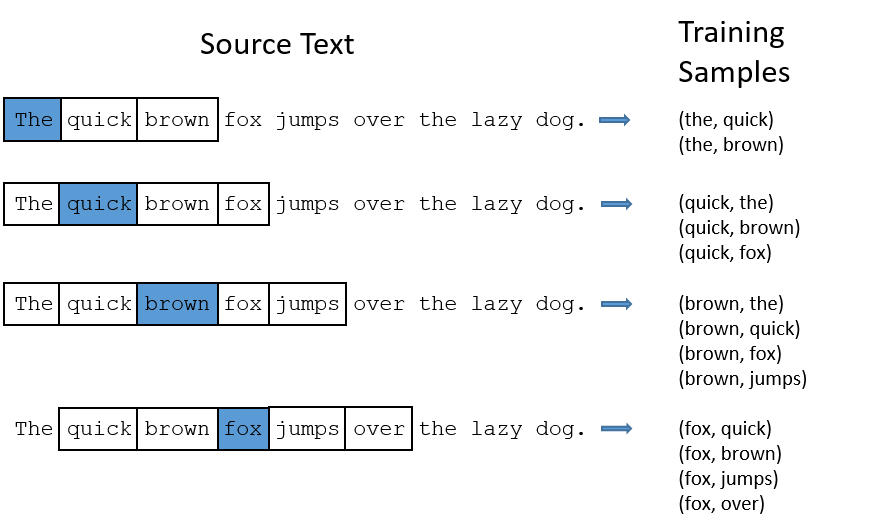
\includegraphics[scale = 0.45]{static/figures/skipgram_sample.png} 
\caption{Παράδειγμα δειγματοληψίας για την εκπαίδευση του μοντέλου \en{SkipGram} \cite{word2vec}}
\label{figure1.2}
\end{figure}

Οι λέξεις εισόδου αναπαριστώνται ως ένα διάνυσμα \(1 \times N\), όπου \(N\) το πλήθος των
λέξεων του λεξιλογίου. Το διάνυσμα αυτό έχει την τιμή ````1\'''' στη θέση που αντιστοιχεί στη 
λέξη εισόδου και ````0'''' αλλού. Η έξοδος του νευρωνικού είναι επίσης ένα \(1 \times N\)
διάνυσμα που σε κάθε θέση περιέχει την πιθανότητα να επιλέξουμε τυχαία τη λέξη στην οποία 
αντιστοιχεί η θέση αυτή. Στο παρακάτω Σχήμα (\ref{figure1.3}) φαίνεται η αρχιτεκτονική
του νευρωνικού, αν η λέξη εισόδου είναι ````\en{ants}'''' (μτφ. μυρμήγκια).

\begin{figure}[!ht] \centering
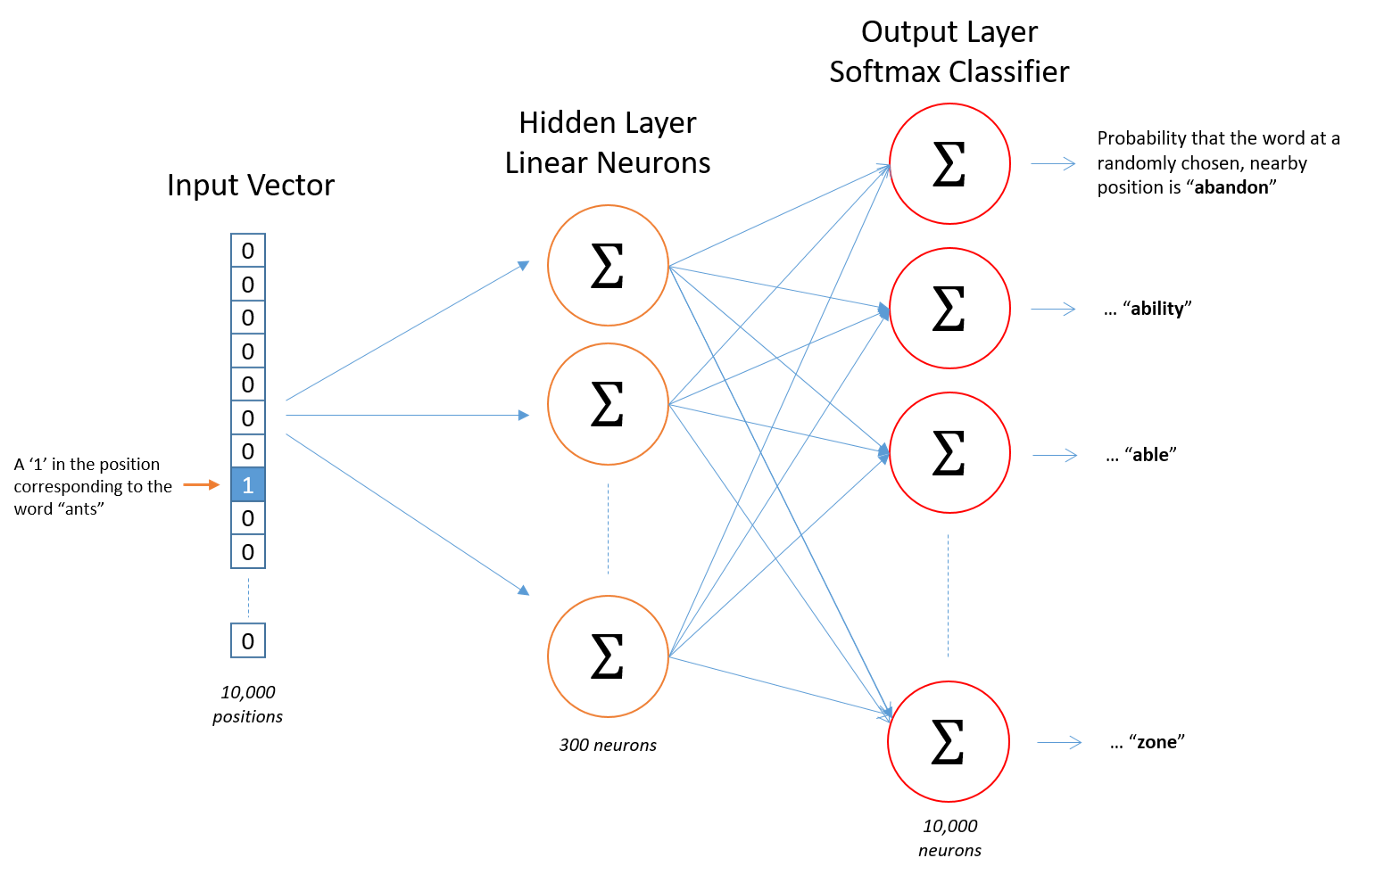
\includegraphics[scale = 0.3]{static/figures/skipgram_nn.png} 
\caption{Δομή του νευρωνικού του μοντέλου \en{SkipGram} \cite{word2vec}}
\label{figure1.3}
\end{figure}

Για το κρυφό στρώμα, δεν υπάρχει συνάρτηση ενεργοποίησης (\en{activation function}), ωστόσο 
στην έξοδο χρησιμοποιείται \en{softmax}. Υπενθυμίζεται ότι η συνάρτηση \en{softmax} είναι
μια συνάρτηση κανονικοποίησης, η οποία παίρνει σαν είσοδο ένα διάνυσμα \(1 \times K\) 
και το κανονικοποιεί σε μια κατανομή πιθανότητας \(K\) ενδεχομένων:

\begin{equation}
    \en{\sigma(\textbf{z})_i = \frac{e^{z_i}}{\sum_{j=1}^{K} e^{z_j}}}
\end{equation}

για \(i=1,\cdots,K\) και \(\textbf{z} = (z_1,\cdots,z_K) \in \mathbb{R}^K\)

Ουσιαστικά, η συνάρτηση \en{softmax} κανονικοποιεί τα στοιχεία του διανύσματος έτσι ώστε
να έχουν μοναδιαίο άθροισμα.

Έστω οτι επιλέχθηκε να αναπαραστήσουμε τις λέξεις με 300 διαστάσεις. Το κρυφό στρώμα
θα αναπαρασταθεί με έναν \(10000 \times 300\) πίνακα (10000 λέξεις στο λεξιλόγιο επί
300 διαστάσεις αναπαράστασης). Ο αριθμός διαστάσεων αναπαράστασης αποτελεί και αυτός
παράμετρο του μοντέλου. Στο τέλος, οι γραμμές του πίνακα αυτού θα είναι οι αναπαραστάσεις
των λέξεων. Στην περίπτωση των γράφων, το κρυφό στρώμα αναπαριστάται από έναν πίνακα
διαστάσεων \(N \times d\), όπου \(N\) το πλήθος των κόμβων του δικτύου και \(d\) ο αριθμός
διαστάσεων που έχει δοθεί σαν παράμετρος του αλγορίθμου. Η τεχνική \en{DeepWalk} 
χρησιμοποιεί αυτή τη λογική, ωστόσο η ακριβής λειτουργία της είναι παρόμοια με μια άλλη
τεχνική, τη \en{Node2Vec} \cite{node2vec}, η οποία εξηγείται σε επόμενη παράγραφο.


\subsection{Aναπαράσταση χωρίς τη χρήση τυχαίων περιπάτων}

Η εκμάθηση αναπαραστάσεων γράφων χωρίς τη χρήση τυχαίων περιπάτων βασίζεται στην εφαρμογή
τεχνικών βαθιάς μάθησης απευθείας στον γράφο ή στον πίνακα γειτνίασης ενός γράφου. Παρακάτω
αναφέρονται ονομαστικά κάποιες τεχνικές χωρίς επεξήγηση, μιας και κάτι τέτοιο ξεφεύγει από
τα πλαίσια της εργασίας.

\begin{itemize}
    \item \textbf{\en{Autoencoder}} (μτφ. Αυτοκωδικοποιητής): Κωδικοποιεί τον γράφο 
    σε ένα χώρο με τον κωδικοποιητή και τον αποκωδικοποιεί με τον αποκωδικοποιτή. Στόχος
    είναι η ελαχιστοποίηση του σφάλματος εισόδου-εξόδου \cite{pan2018adversarially}.
    \item \textbf{\en{Deep Neural Network}} (μτφ. Βαθύ Νευρωνικό Δίκτυο):  Χρησιμοποιεί \en{Convolutional Neural 
    Networks} (\en{CNN's}) (μτφ. Συνελικτικό Νευρωνικό Δίκτυο) για εκμάθηση
    αναπαραστάσεων από γράφους \cite{pmlr-v48-niepert16}.
\end{itemize}

\subsection{Από την αναπαράσταση κόμβων στην αναπαράσταση ακμών}

Το πρόβλημα της αναπαράστασης γράφων μπορεί, κατά περίπτωση, να οριστεί ως προς την είσοδο
και την έξοδο, με πολλούς τρόπους, ανάλογα με τις προϋποθέσεις της εκάστοτε τεχνικής που 
θα εφαρμοστεί, αλλά και ανάλογα με τον τύπο προβλήματος που πρόκειται να επιλύσουν
\cite{cai2017comprehensive}:

\begin{itemize}
    \item Είσοδος: \begin{itemize}
                        \item Ομογενής γράφος
                        \item Ετερογενής γράφος
                        \item Γράφος με χαρακτηριστικά κόμβων/ακμών
                        \item Γράφος κατασκευασμένος από μη-σχεσιακά δεδομένα
                   \end{itemize}
    \item Έξοδος: \begin{itemize}
                        \item Αναπαράσταση κόμβων
                        \item Αναπαράσταση ακμών
                        \item Υβριδική αναπαράσταση
                        \item Αναπαράσταση ολόκληρου γράφου
                  \end{itemize}
\end{itemize}

Για τους σκοπούς της εργασίας αυτής, για λόγους απλότητας, αποτελεσματικότητας και δυνατότητας 
βελτιστοποίησης επιλέχθηκε η χρήση αναπαράστασης κόμβων, και έπειτα κατασκευή της
αναπαράστασης ακμών από την αναπαράσταση κόμβων. Για την διεργασία αυτή, υπάρχουν διάφοροι
τελεστές \cite{node2vec}, οι οποίοι κατά περίπτωση διερευνώνται και επιλέγεται ο βέλτιστος για
τα εκάστοτε δεδομένα:

\begin{itemize}
    \item \en{Hadamard} : \begin{equation}
                            [f(u) \boxdot f(v)]_i = f_{i}(u) \ast f_{i}(v)
                          \end{equation} 
    \item \en{Average} : \begin{equation}
                            [f(u) \boxplus f(v)]_i = \frac{f_{i}(u) + f_{i}(v)}{2}   
                         \end{equation}
    \item \en{Weighted-L1} : \begin{equation}
                                \parallel f(u) \dot f(v) \parallel_{\Bar{1}_{i}} = 
                                |f_{i}(u) - f_{i}(v)|
                            \end{equation}
    \item \en{Weighted-L2} : \begin{equation}
                                \parallel f(u) \dot f(v) \parallel_{\Bar{2}_{i}} = 
                                |f_{i}(u) - f_{i}(v)|^2
                             \end{equation}
\end{itemize}

όπου \(f(u), f(v)\) η αναπαράσταση των κόμβων \(u, v\) αντίστοιχα και \(f_{i}(u)\) η 
\(i\)-οστή συνιστώσα της αναπαράστασης του κόμβου \(u\)


\subsection{Μηχανική μάθηση και ταξινόμηση}

Το πρόβλημα της ταξινόμησης είναι από τα πιο δημοφιλή για χρήση μηχανικής μάθησης. 
Ανήκει στην οικογένεια της επιβλεπόμενης (\en{supervised}) μηχανικής μάθησης, και στόχος
είναι η ανάπτυξη ενός μοντέλου που θα κατηγοριοποιεί ορθά τα δεδομένα εισόδου σε
μια σειρά κλάσεων. Το μοντέλο δηλαδή παίρνει σαν είσοδο μια παρατήρηση και στην έξοδο
βγάζει την κατηγορία στην οποία εμπίπτει αυτή η παρατήρηση. Η έξοδος δηλαδή είναι διακριτή
τιμή. Μια παραλλαγή του προβλήματος αποτελεί η Παλινδρόμηση (\en{Regression})
όπου η έξοδος είναι μια συνεχής τιμή, συνήθως μια πιθανότητα η είσοδος να εμπίπτει σε μια 
συγκεκριμένη κλάση. Θέτοντας ένα όριο π.χ. 0,5 στην έξοδο, οι τεχνικές παλινδρόμησης
χρησιμοποιούνται για προβλήματα ταξινόμησης. Για όριο (\en{Threshold}) ίσο με 0,5 
θεωρείται ότι άν η έξοδος δώσει μια πιθανότητα άνω από 0,5 μια παρατήρηση \(x\) 
να ανήκει στην κλάση \(y\), τότε η παρατήρηση ανήκει στην κλάση αυτή, και ούτω καθεξής (κ.ο.κ.).

Ένα πρόβλημα δυαδικής ταξινόμησης ή παλινδρόμησης είναι ένα πρόβλημα στο οποίο υπάρχουν 
2 δυνατές κλάσεις. Στα πλαίσια της εργασίας θα χρησιμοποιηθεί μια τεχνική παλινδρόμησης,
η \en{Logistic Regression with Cross-Validation} (μτφ. Λογιστική Παλινδόμηση με διασταυρωμένη επικύρωση) για την ανάπτυξη ενός μοντέλου Ταξινόμησης.

\subsubsection{Λογιστική παλινδρόμηση}

Το λογιστικό μοντέλο χρησιμοποιείται για να μοντελοποιήσει την πιθανότητα εμφάνισης ενός
γεγονότος δυαδικής φύσεως, όπως είναι η νίκη/ήττα, επιτυχία/αποτυχία κ.ο.κ. Οι πιθανές
 εκβάσεις μπορούν να είναι και περισσότερες από 2, ωστόσο το μοντέλο δίνει μια πιθανότητα
(από 0 ως 1) κάποια παρατήρηση να εμπίπτει σε κάθε κλάση, και οι πιθανότητες κάθε κλάσης
για κάθε παρατήρηση έχουν μοναδιαίο άθροισμα.

Η λογιστική παλινδρόμηση \cite{10.1001/jama.2016.7653} αποτελεί ένα στατιστικό μοντέλο που
στη βασική του μορφή υλοποιεί την προαναφερθείσα λειτουργία. Από μαθηματικής άποψης, το 
λογιστικό μοντέλο έχει μια εξαρτημένη μεταβλητή με δύο πιθανές τιμές που ανήκουν στο δισύνολο \(\{0, 1\}\).
Ο λογάριθμος της πιθανότητας της τιμής ````1'''' είναι ένας γραμμικός (ή μη) συνδυασμός ενός
αριθμού ανεξάρτητων μεταβλητών που ονομάζονται μεταβλητές πρόβλεψης (\en{predictors}). Οι
ανεξάρτητες μεταβλητές μπορούν να είναι είτε δυαδικές είτε συνεχείς. Η τελική πιθανότητα της
τιμής ````1'''' μπορεί να είναι από 0 (σίγουρα η τιμή ````0'''') μέχρι και 1 (σίγουρα η τιμή ````1''''). Η
συνάρτηση που μετατρέπει το λογάριθμο σε πιθανότητα είναι η λογιστική συνάρτηση
(\ref{logistic_func}), αλλά χρησιμοποιούνται και μοντέλα με διαφορετικές σιγμοειδείς
συναρτήσεις. Το κύριο χαρακτηριστικό των λογιστικών μοντέλων είναι πως η αύξηση μίας
ανεξάρτητης μεταβλητής επηρεάζει την τελική πιθανότητα κατά σταθερό ρυθμό, και κάθε 
ανεξάρτητη μεταβλητή έχει την δική της παράμετρο.

\begin{equation}
    S(x) = \frac{1}{1 + e^{-x}} = \frac{e^x}{e^{x} + 1}
    \label{logistic_func}
\end{equation}

\begin{figure}[!ht] \centering
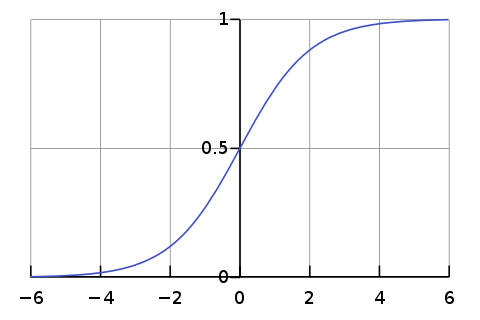
\includegraphics[scale = 0.6]{static/figures/logistic_curve.png} 
\caption{Τυπική μορφή λογιστικής συνάρτησης \cite{10.1001/jama.2016.7653}}
\label{figure1.4}
\end{figure}

Στην περίπτωση του δυαδικού μοντέλου λογιστικής παλινδρόμησης, η εξαρτημένη μεταβλητή είναι
κατηγορική, δηλαδή όπως προαναφέρθηκε έχει δύο πιθανές τιμές, που αναφέρονται και ως κλάσεις.
Το λογιστικό μοντέλο ωστόσο απλώς δίνει μια πιθανότητα σε κάθε μία από τις δύο πιθανές
κλάσεις και από μόνο του δεν αποτελεί ταξινομητή. Για να χρησιμοποιηθεί σαν ταξινομητής
συνήθως επιλέγεται όπως αναφέραμε ένα κατώφλι (\en{threshold}). Οι συντελεστές του μοντέλου
δεν υπολογίζονται με κάποια συγκεκριμένη μεθοδολογία, και για το λόγο αυτό στα πλαίσια της
εργασίας χρησιμοποιήθηκε η τεχνική της διασταυρωμένης επικύρωσης (\en{Cross Validation}).
Η τεχνική αυτή καθιστά δυνατή την αυτόματη βελτιστοποίηση των παραμέτρων του μοντέλου.
Ο τρόπος λειτουργίας της τεχνική αυτής ξεφεύγει από τα πλαίσια της εργασίας αυτής.

\subsection{Επικύρωση μοντέλων μηχανικής μάθησης}

Για την ορθή ανάπτυξη μοντέλων με χρήση μηχανικής μάθησης, είναι απαραίτητη η χρήση κάποιων
μετρικών για την διαπίστωση της αποτελεσματικότητας του μοντέλου υπο ανάπτυξη. Οι μετρικές
αφορούν την περίπτωση της επιβλεπόμενης μηχανικής μάθησης, όπου οι ορθές τιμές εξόδου 
κατά το στάδιο της εκπαίδευσης είναι γνωστές. Συνήθως χρησιμοποιείται μια συνάρτηση που 
συγκρίνει τις εξόδους του μοντέλου με τις ορθές τιμές και δίνει κάποια τιμή που όσο 
μεγαλύτερη είναι τόσο πιο ακριβές είναι το μοντέλο. 

Για την περίπτωση των ταξινομητών και ειδικότερα της δυαδικής ταξινόμησης για την έξοδο
του μοντέλου υπάρχουν οι εξής περιπτώσεις σχετικά με την ορθότητα του αποτελέσματος για
μία παρατήρηση:

\begin{itemize}
    \item Αληθές Θετικό (\en{True Positive - TP}): Ο ταξινομητής κατέταξε την παρατήρηση
    στην κλάση ````1'''' ορθά, δηλαδή η παρατήρηση όντως ανήκει στην κλάση ````1''''
    \item Ψευδές Θετικό (\en{False Positive - FP}): Ο ταξινομητής κατέταξε την παρατήρηση
    στην κλάση ````1'''' λανθασμένα, δηλαδή η παρατήρηση ανήκει στην κλάση ````0''''
    \item Αληθές Αρνητικό (\en{True Negative - TN}): Ο ταξινομητής κατέταξε την παρατήρηση
    στην κλάση ````0'''' ορθά, δηλαδή η παρατήρηση όντως ανήκει στην κλάση ````0''''
    \item Ψευδές Αρνητικό (\en{False Negative - FN}): Ο ταξινομητής κατέταξε την παρατήρηση
    στην κλάση ````0'''' λανθασμένα, δηλαδή η παρατήρηση ανήκει στην κλάση ````1''''
\end{itemize}

Από τα παραπάνω σχηματίζεται ο \en{Confusion Matrix} (μτφ. Πίνακας Σύγχυσης) που στην περίπτωση
της δυαδικής ταξινόμησης είναι ένας \(2 \times 2\) πίνακας. Στην εικόνα \ref{figure1.5} 
δίνεται ένα παράδειγμα όπου οι κλάσεις αντί για ````0'''' και ````1'''' είναι ````\en{Yes}'''' και ````\en{No}''''.

\begin{figure}[!ht] \centering
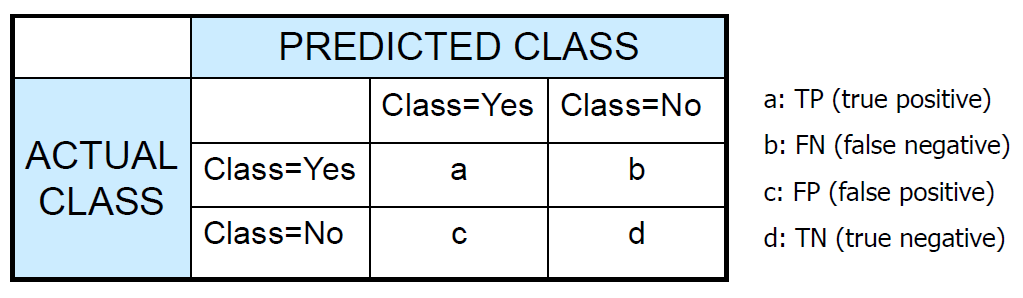
\includegraphics[scale = 0.6]{static/figures/conf_matrix.png} 
\caption{Τυπική μορφή πίνακα σύγχυσης \cite{DataMining}}
\label{figure1.5}
\end{figure}

Επίσης σχηματίζεται και η μετρική (\en{Accuracy}) (μτφ. Ακρίβειας), που δίνει το ποσοστό των
ορθά ταξινομημένων παρατηρήσεων σε σχέση με το πλήθων των ταξινομήσεων:

\begin{equation}
    Accuracy = \frac{TP + TN}{TP + TN + FP + FN}
\end{equation}

Η μετρική \en{Accuracy}, ενώ είναι πολύ δημοφιλής, υπάρχουν περιπτώσεις στις οποίες δίνει λανθασμένη εικόνα για την
ποιότητα του μοντέλου. Για παράδειγμα για ένα σύνολο παρατηρήσεων που έχει 9990 εγγραφές
που ανήκουν στην κλάση ````0'''' και 10 εγγραφές που ανήκουν στην κλάση ````1'''', αν το μοντέλο 
ταξινομήσει όλες τις παρατηρήσεις στην κλάση ````0'''' δίνεται μια τιμή \en{Accuracy} = \(99.9\%\),
που ενώ είναι μια πολύ καλή τιμή ακρίβειας, το μοντέλο υπό ανάπτυξη είναι πολύ κακό.

Υπάρχουν και μερικές μετρικές πολωμένες ως προς μια κατηγορία αποτελεσμάτων. Για παράδειγμα,
η μετρική \en{Precision} (μτφ. Ευστοχίας), είναι πολωμένη ως προς τα \en{TP,
FP}:

\begin{equation}
    Precision = \frac{TP}{TP + FP}
\end{equation}

H μετρική \en{Recall} (μτφ. Ανάκλησης), είναι πολωμένη ως προς τα \en{TP, FN}:

\begin{equation}
    Recall = \frac{TP}{TP + FN}
\end{equation}

Από τις δύο τελευταίες μετρικές προκύπτει η μετρική ````\en{F1-Score}'''' που τις συνδυάζει 
ως τον αρμονικό μέσο, και όχι τον αριθμητικό. Επιλέγεται ο αρμονικός μέσος επειδή ````τιμωρεί''''
περισσότερο τις ακραίες περιπτώσεις. Για παράδειγμα, σε έναν ταξινομητή με εντελώς τυχαία
πρόβλεψη θα δίνει μια ακρίβεια περίπου \(50\%\). Για τις ανάγκες του παραδείγματος θεωρείται
πως η τιμή της \en{Recall} = 0 και \en{Precision} = 1. Αν επιλεγόταν ο αριθμητικός μέσος
θα εδίνε μια τιμή 0.5. Ο αρμονικός μέσος δίνει μια τιμή 0, που αντιπροσωπεύει καλύτερα την
αποτελεσματικότητα του μοντέλου που είναι μηδαμινή, αφού ουσιαστικά αγνοεί την είσοδο και
````προβλέπει'''' τυχαία. Η τιμή της μετρικής δίνεται από τον τύπο:

\begin{equation}
    F1\_Score = 2 * \frac{Recall * Precision}{Precision + Recall}
\end{equation}

Μια ακόμα εξαιρετικά δημοφιλής είναι οι καμπύλες \en{Receiver Operating
Characteristics (ROC)} (μτφ. Χαρακτηριστικά Λειτουργίας Δέκτη). Εμφανίστηκαν τη δεκαετία του
1950 στο πεδίο της ανάλυσης σημάτων για την ανάλυση θορυβοδών σημάτων \cite{DataMining}. 

\subsubsection{Καμπύλες \en{ROC}}

Οι καμπύλες \en{ROC} αναπαριστούν τις \en{TP} παρατηρήσεις στον άξονα \en{y} ως προς τις
\en{FP} παρατηρήσεις, στον άξονα \en{x}. Η επίδοση ενός μοντέλου ταξινόμησης αναπαρίσταται 
ως ένα σημείο στην καμπύλη. Αλλάζοντας το κατώφλι του αλγορίθμου, αλλάζει και η θέση του
σημείου. Το σημείο [0,0] αντιπροσωπεύει τιμή κατωφλίου 1, δηλαδή όλες οι παρατηρήσεις
ταξινομούνται στην κλάση ````0'''', ενώ το [1,1] το αντίστροφο, δηλαδή όλες οι παρατηρήσεις
ταξινομούνται στην κλάση ````1''''. Το σημείο [0,1] είναι το ιδανικό, που αντιπροσωπεύει την
περίπτωση όπου όλες οι παρατηρήσεις ταξινομήθηκαν σωστά, ενώ η κύρια διαγώνιος αντιπροσωπεύει
έναν τυχαίο ταξινομητή. Αν τα σημεία της καμπύλης είναι κάτω από την κύρια διαγώνιο, 
τότε ο ταξινομητής ταξινομεί τις παρατηρήσεις ανάποδα. Τέλος, η μετρική \en{Area Under Curve Score (AUC-Score)} (μτφ. Μετρική Περιοχής Κάτω από την Καμπύλη)
δίνει το ποσοστό της επιφάνειας που βρίσκεται κάτω από την καμπύλη 
ως προς την συνολική επιφάνεια. Στην \ref{figure1.6} δίνεται ένα παράδειγμα καμπύλης 
\en{ROC}.

\begin{figure}[!ht] \centering
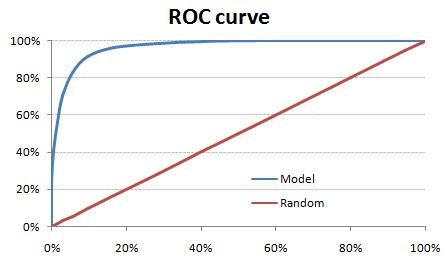
\includegraphics[scale = 1]{static/figures/ROC.jpg} 
\caption{Ενδεικτική μορφή καμπύλης \en{ROC} \cite{DataMining}}
\label{figure1.6}
\end{figure}


\section{Τεχνικές εξαγωγής αναπαραστάσεων}

Όπως έχει γίνει ήδη αντιληπτο, για να χρησιμοποιηθεί μηχανική μάθηση σε ένα πρόβλημα με
δεδομένα σε μορφή γράφου θα πρέπει πρώτα ο τελευταίος να μετατραπεί σε μια πιο παραδοσιακή
μορφή συνόλου δεδομένων, αυτή που αντιπροσωπεύει ένα σύνολο παρατηρήσεων/σημείων. Για τον
σκοπό αυτό έχουν αναπτυχθεί πολλές τεχνικές, ωστόσο στην εργασία αυτή επιλέχθηκαν και
χρησιμοποιήθηκαν 3 συγκεκριμένες οι οποίες θα αναλυθούν στη συνέχεια. Και οι τρείς τεχνικές
χρησιμοποιούν τεχνικές μη-επιβλεπόμενης μηχανικής μάθησης.

\subsection{\en{Node2Vec}} \label{n2v}

Η πρώτη τεχνική εξαγωγής αναπαραστάσεων κόμβων \en{node features}) από γράφο που επιλέχθηκε
είναι η \en{Node2Vec} \cite{node2vec}. Η βασική ιδέα που υλοποιεί αυτή η τεχνική είναι η
εξής: κόμβοι που βρίσκονται ````κοντά'''' σε ένα γράφο αναπαριστώνται με n-διάστατα σημεία στο
n-διάστατο χώρο που θα είναι εξ' ίσου ````κοντά''''. Διατηρείται δηλαδή η ιδιότητα των γειτονικών
σημείων κατά τη μετάβαση από τη μια μορφή αναπαράστασης των δεδομένων (γράφος) στην άλλη
(σημεία στο χώρο). Η τεχνική αυτή αποτελεί εξέλιξη μιας προϋπάρχουσας τεχνικής, της
\en{DeepWalk} \cite{DeepWalk}.

Η \en{Node2Vec} αρχικά δειγματοληπτεί τον γράφο πραγματοποιώντας ````τυχαίους περιπάτους'''' πάνω
σε αυτόν. Ξεκινώντας από ένα τυχαίο κόμβο, έστω \(u_i\), διασχίζει τον γράφο από κόμβο σε κόμβο με
τυχαία σειρά, σχηματίζοντας ένα μονοπάτι συγκεκριμένου μήκους \(l\), το οποίο αποτελεί το
δείγμα. Το αποτέλεσμα είναι μια αλληλουχία κόμβων \({u_1, u_2,...,u_k}\). Αυτή η διαδικασία
επαναλαμβάνεται \(k\) φορές για κάθε κόμβο. Η σημασία του \(l\) και του \(k\) είναι πολύ
υψηλή. Όσο αυξάνεται το \(k\), τόσο περισσότερο εξερευνάται ο γράφος, και τόσο περισσότερα
μονοπάτια δημιουργούνται. Όσο αυξάνεται το \(l\), τόσο αυξάνει το μήκος κάθε περιπάτου, και
άρα όλο και πιο μακρινοί κόμβοι λαμβάνονται υπόψιν ως ````γειτονικοί''''. Στη συνέχεια, το δείγμα
δίνεται ως είσοδος σε ένα μοντέλο \en{SkipGram} (Παράγραφος \ref{SkipGram}).

\subsubsection{Παράμετροι \en{Node2Vec}}

Ο \en{Node2Vec} δειγματοληπτεί τον γράφο όπως προαναφέραμε, και επιστρέφει έναν πίνακα 
\(N \times d\), όπου η κάθε γραμμή αντιστοιχεί σε κάθε κόμβο του δικτύου. Για να το πετύχει
αυτό δέχεται κάποιες παραμέτρους:

\begin{itemize}
    \item Αριθμός περιπάτων από κάθε κόμβο
    \item Μήκος κάθε περιπάτου
    \item \en{Q}, όπου \(1/Q\) η πιθανότητα κατά τον περίπατο να μεταπηδήσει 
    από έναν κόμβο \(u_i\) σε έναν γειτονικό κόμβο \(u_j\)
    \item \en{P}, όπου \(1/P\) η πιθανότητα κατά τον περίπατο να μεταπηδήσει 
    από έναν κόμβο \(u_i\) στον ίδιο κόμβο \(u_i\)
\end{itemize}

Επί της ουσίας, οι παράμετροι \(Q,P\) ρυθμίζουν την εστίαση του αλγορίθμου στην διατήρηση
των τοπικών γειτονιών ή της γενικότερης δομής του γράφου. Τέλος, τα βάρη των ακμών
λαμβάνονται υπ' όψιν, οπότε η τελική πιθανότητα μετάβασης για κάθε κόμβο είναι συνάρτηση των
3 παραμέτρων (\(Q,P,w\)). Το Σχήμα \ref{figure1.7} απεικονίζει ένα παράδειγμα λειτουργίας
του \en{Node2Vec} για \(d = 2\).

\begin{figure}[!ht] \centering
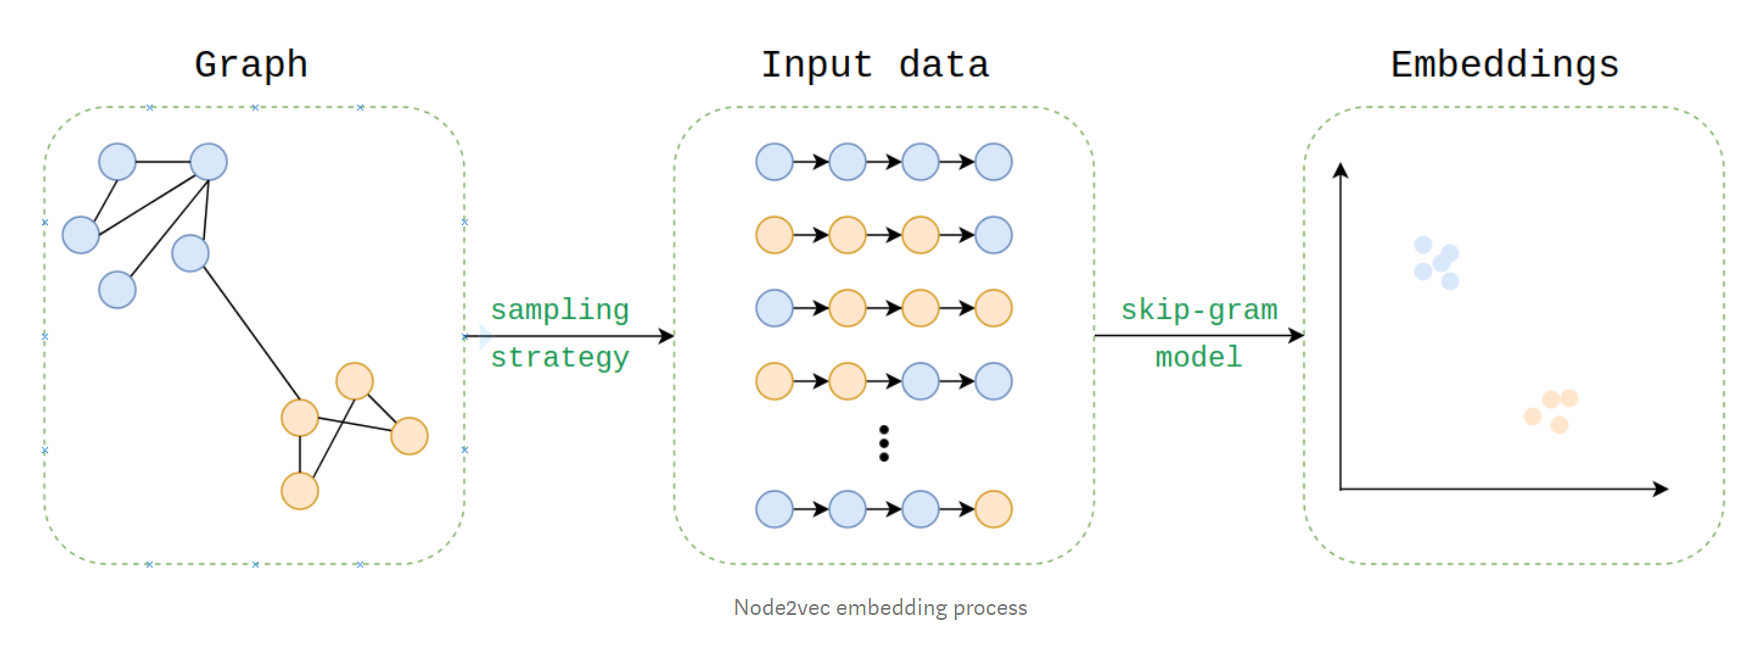
\includegraphics[scale = 0.3]{static/figures/n2v_figure.png} 
\caption{Τρόπος λειτουργίας \en{Node2Vec} για \(d = 2\) \cite{Node2VecImpl}}
\label{figure1.7}
\end{figure}

\subsection{\en{CTDNE}} \label{CTDNE}

Η δεύτερη τεχνική εξαγωγής αναπαραστάσεων είναι η \en{CTDNE - Continuous-Time Dynamic
Network Embeddings} \cite{CTDNE}. Η τεχνική αυτή ενσωματώνει τη χρονική παράμετρο στο
πρόβλημα εξαγωγής αναπαραστάσεων γράφου. Αφορά γράφους που αντιπροσωπεύουν ένα πρόβλημα
παραμετροποιημένο ως προς τον χρόνο. Πρακτικά στις περισσότερες εφαρμογές αυτό υλοποιείται
με τα βάρη των ακμών, όπου το βάρος μιας ακμής εμπεριέχει την πληροφορία για το πότε
δημιουργήθηκε.

Η \en{CTDNE} έχει παρόμοια λειτουργία με την \en{Node2Vec}, ωστόσο διαφέρει στον τρόπο
δειγματοληψίας τυχαίων περιπάτων. Εισάγει την έννοια των χρονικών τυχαίων περίπατων 
\({u_1, u_2,\cdots,u_k}\), όπου \(T(u_i,u_{i+1}) \leq T(u_{i+1},u_{i+2})\), δηλαδή η χρονική
στιγμή που δημιουργήθηκε η ακμή μεταξύ των κόμβων (\(u_i,u_{i+1}\)) είναι πρεσβύτερη από τη
χρονική στιγμή που δημιουργήθηκε η ακμή μεταξύ των κόμβων (\(u_{i+1},u_{i+2}\)). 
Οι δημιουργοί της τεχνικής δίνουν 3 επιλογές ως προς το όσο πολωμένη θα είναι η επιλογή
αρχικών ακμών ως προς τον χρόνο(\(Pr(e)\) η πιθανότητα να επιλεγεί η ακμή \(e\)):

\begin{itemize}
    \item Μη πολωμένη, όπου \(Pr(e) = 1/|E_T|\)
    \item Πολωμένη\begin{itemize}
            \item Εκθετικά, όπου 
            
            \begin{equation}
                Pr(e) = \frac{exp[T(e) - t_{min}]}
                {\sum_{e^{'} \in E_T} exp[T(e^{'}) - t_{min}]}
            \end{equation}
            
            και \(t_{min}\) η παλαιότερη χρονική στιγμή που υπάρχει στον γράφο. 
            Αυτή η κατανομή είναι σημαντικά πολωμένη ως προς τις νεότερες ακμές
            
            \item Γραμμικά, όπου
            
            \begin{equation}
                Pr(e) = \frac{\eta(e)}{\sum_{e^{'} \in E_T} \eta(e^{'})}
            \end{equation}
            
            και \(\eta(e)\) μια συνάρτηση που συσχετίζει κάθε ακμή με ένα δείκτη, και η
            παλαιότερη ακμή όλων έχει \(\eta(e) = 1\)
            
        \end{itemize}
\end{itemize}

Λόγω της φύσης του αλγορίθμου, είναι βέλτιστο να διατυπωθούν οι παράμετροι που δέχεται ο
αλγόριθμος ως εξής:

\begin{itemize}
    \item Αριθμός περιπάτων από κάθε κόμβο (\(R\))
    \item Μήκος κάθε περιπάτου (\(L\))
    \item Παράθυρο περιβάλλοντος (\en{Context Window}, \(\omega\))
    \item Αριθμός παραθύρων περιβάλλοντος (\(\beta\))
    \item Τρόπος επιλογής ακμής (Πολωμένη Εκθετικά/Γραμμικά, Μη Πολωμένη)
\end{itemize}

Σε αντίθεση με τη \en{Node2Vec}, δεν είναι χρήσιμο να ορίσουμε ένα μήκος περιπάτου, αλλά ένα
εύρος αποδεκτών μηκών μονοπατιού, αφού στην τεχνική αυτή δίνεται βάρος στην χρονική
εγκυρότητα του μονοπατιού. Ειδικότερα για την παράμετρο \(\beta\), σύμφωνα με το
\cite{CTDNE} ορίζεται ως συνάρτηση των άλλων παραμέτρων:
\begin{equation} \label{2.19}
    \beta = R \times N \times ( L - \omega + 1)
\end{equation}
όπου \(N\) ο αριθμός των κόμβων του γράφου.

\subsection{\en{GraphSAGE}} \label{gsage}

Η τρίτη τεχνική εξαγωγής αναπαραστάσεων που επιλέχθηκε είναι η \en{GraphSage}
\cite{GraphSAGE}. Η ειδοποιός διαφορά ανάμεσα σε αυτή και στις προηγούμενες
είναι ότι η \en{GraphSage} χρησιμοποιεί τα χαρακτηριστικά των κόμβων (\en{node attributes})
για να παράξει αναπαραστάσεις αυτών (\en{node embeddings}).

Οι προηγούμενες τεχνικές αποτελούν μεταγωγικές (\en{transductive}) μεθόδους, δηλαδή εξάγουν
αναπαραστάσεις από ένα δεδομένο και σταθερό γράφο. Η \en{GraphSage} αποτελεί μια επαγωγική
(\en{inductive}) μέθοδο εξαγωγής αναπαραστάσεων, που σημαίνει ότι λειτουργεί και σε δυναμικά
περιβάλλοντα, παράγοντας αναπαραστάσεις για νέους κόμβους χωρίς την ανάγκη επανεκπαίδευσης
του συστήματος. Αυτό πετυχαίνεται με τη χρήση συναθροιστικών συναρτήσεων 
(\en{aggregator functions}), των οποίων ο ρόλος είναι να συναθροίζουν πληροφορία για κάθε
κόμβο από τους γείτονές τους. Τα βάρη των συναθροιστικών συναρτήσεων μπορεί να είναι 
σταθερά ή να προκύπτουν μέσα από εκπαίδευση, ανάλογα με την συνάρτηση.

Για την εξαγωγή αναπαραστάσεων με συναθροιστικές συναρτήσεις, αρχικά παράγονται
αναπαραστάσεις για κάθε κόμβο από τα χαρακτηριστικά του. Έπειτα, για κάθε κόμβο, παράγεται
μια αναπαράσταση αυτού βάσει της ````γειτονιάς'''' του, δηλαδή όσων κόμβων έχουν απόσταση \(K\)
από αυτόν \(K \in [1,n)\) και συνενώνεται με την υπάρχουσα αναπαράσταση για τον κόμβο αυτό.
Τέλος το συνολικό διάνυσμα της αναπαράστασης μπαίνει σαν είσοδο σε ένα νευρωνικό δίκτυο,
ώστε να ανανεωθεί η τελική αναπαράσταση του κόμβου. Αφού η διαδικασία επαναληφθεί για κάθε
κόμβο, κανονικοποιούνται οι αναπαραστάσεις ώστε να έχουν μοναδιαίο άθροισμα.
Παρουσιάζεται στο Σχήμα \ref{figure1.8} ο αλγόριθμος σε ψευδοκώδικα όπως δίνεται στο
\cite{GraphSAGE}.

\begin{figure}[!ht] \centering
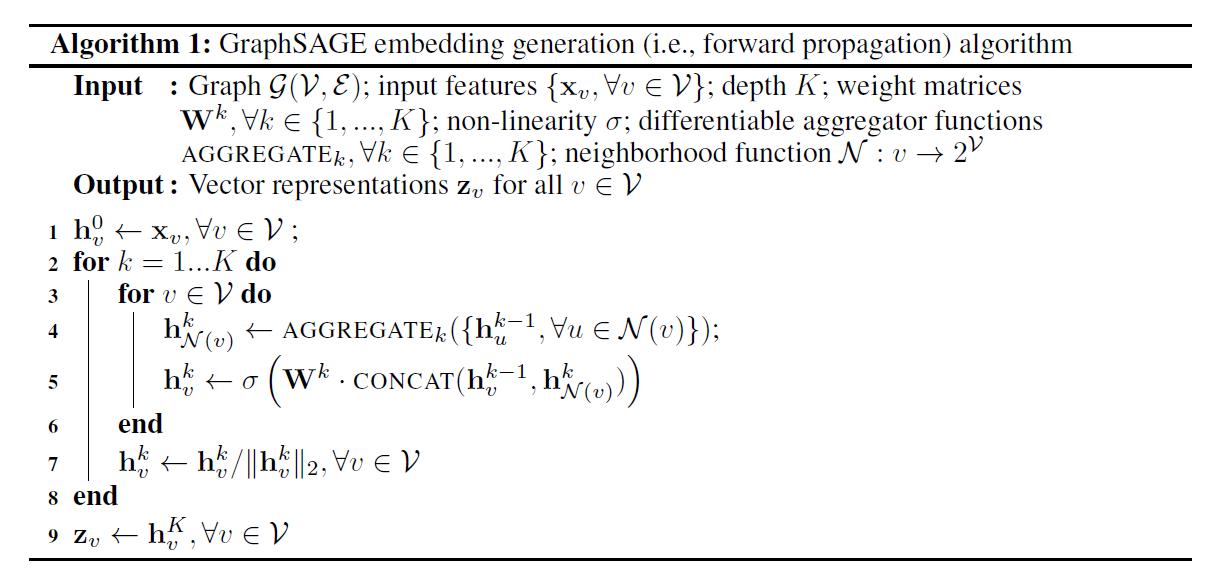
\includegraphics[scale = 0.5]{static/figures/GSAGE_algo.png} 
\caption{Αλγόριθμος  \en{GraphSage} παραγωγής  αναπαραστάσεων κόμβων \cite{GraphSAGE}}
\label{figure1.8}
\end{figure}

Για την βελτιστοποίηση των βαρών των συναρτήσεων συνάθροισης χρειαζόμαστε μια συνάρτηση
απώλειας (\en{loss function}), η οποία να ικανοποιεί τον περιορισμό οτι γειτονικοί κόμβοι
θα πρέπει να έχουν παρόμοιες αναπαραστάσεις και απομακρυσμένοι κόμβοι να έχουν
αρκετά διαφορετικές αναπαραστάσεις. Η συνάρτηση που προτείνεται στο
\cite{GraphSAGE} είναι η:

\begin{equation}
    J_{G}(\boldsymbol{z}_{u}) = -\log(\sigma)(\boldsymbol{z}_{u}^{T}\boldsymbol{z}_{v})
    - Q \cdot E_{u_{n}~P_{n}(v)} \log(\sigma(-\boldsymbol{z}_{u}^{T}\boldsymbol{z}_{v_{n}}))
\end{equation}

όπου \(u\) και \(v\) είναι 2 γειτονικοί κόμβοι και η συνάρτηση υπολογίζεται ως προς \(u\).
Ο πρώτος όρος μεγιστοποιεί την ομοιότητα των αναπαραστάσεων των \(u\) και \(v\). Στον δεύτερο
ο όρος \(Q\) είναι ο αριθμός των αρνητικών δειγμάτων (μη γειτονικοί κόμβοι) και \(v_n\) 
ένα αρνητικό δείγμα από μια κατανομή αρνητικών δειγμάτων. Οπότε ο δεύτερος όρος μεγιστοποιεί
τη διαφοροποίηση των μη-γειτονικών κόμβων και \(\sigma\) η σιγμοειδής συνάρτηση. Τέλος,
επισημαίνεται ότι η συνάρτηση αυτή υλοποιεί μια μη-επιβλεπόμενη μέθοδο εκμάθησης,
ωστόσο είναι δυνατό ο χρήστης να υλοποιήσει τον αλγόριθμο σε πλαίσιο επιβλεπόμενης 
εκπαίδευσης.
    \chapter{Μεθοδολογία}

Στο κεφάλαιο αυτό θα αναλυθεί η μεθοδολογία που ακολουθήθηκε για την διεκπεραίωση της εργασίας
αυτής, καθώς και ο λόγος που έγιναν οι συγκεκριμένες επιλογές, τόσο ως προς τις τεχνικές
όσο και τα δεδομένα. Αρχικά θα αναλυθούν τα σύνολα δεδομένων που επιλέχθηκαν, και έπειτα
θα αναλυθεί ο τρόπος δόμησης κάθε τεχνικής.

\section{Δεδομένα}

Για την εργασία αυτή επιλέχθηκαν δύο σύνολα δεδομένων με διαφορετικές ιδιότητες το καθένα. Πρώτο
επιλέχθηκε το \en{CORA Dataset} (μτφ. Σύνολο Δεδομένων) \cite{sen2008collective} και δεύτερο το 
\en{Bitcoin OTC (trust weighted signed network) Dataset} \cite{kumar2016edge} \cite{kumar2018rev2}.

\subsection{\en{CORA dataset}}

To \en{CORA Dataset} δημιουργήθηκε στα πλαίσια μιας προσπάθειας δημιουργίας ενός συνόλου
δεδομένων κατάλληλο για εξέλιξη τεχνικών ταξινόμησης με χρήση μηχανικής μάθησης
\cite{sen2008collective}. Το αρχικό σύνολο δεδομένων αποτελείται από ένα σύνολο 2708
επιστημονικών δημοσιεύσεων, που αποτελούν τους κόμβους. Οι δημοσιεύσεις/κόμβοι είναι κατηγοριοποιημένοι
σε μία από 7 κλάσεις σχετικά με το αντικείμενο τους:

\begin{itemize}
    \item Με βάση την υπόθεση (\en{Case Based})
    \item Γενετικοί Αλγόριθμοι (\en{Genetic Algorithms})
    \item Νευρωνικά Δίκτυα (\en{Neural Networks})
    \item Πιθανοτικές Μέθοδοι (\en{Probabilistic Methods})
    \item Επιβραβευόμενη Μάθηση (\en{Reinforcement Learning})
    \item Εκμάθηση Κανόνων (\en{Rule Learning})
    \item Θεωρία (\en{Theory})
\end{itemize}

Κάθε επιστημονική δημοσίευση (κόμβο) συνοδεύεται από ένα σύνολο χαρακτηριστικών (\en{Node 
attributes}). Κατά το σχεδιασμό του συνόλου δεδομένων, σχηματίστηκε ένα λεξικό με λέξεις που
υπάρχουν στις δημοσιεύσεις και χαρακτηρίζουν το περιεχόμενό τους. Αφαιρέθηκαν δηλαδή αντωνυμίες,
άρθρα, κ.λπ. Τελικά σχηματίστικε ένα σύνολο 1433 μοναδικών λέξεων. Κάθε κόμβος χαρακτηρίζεται
από ένα διάνυσμα 1433 θέσεων, όπου κάθε θέση συμπληρώνεται με "0" ή "1" ανάλογα με το εάν
υπάρχει στη δημοσίευση η λέξη του λεξικού στην οποία αντιστοιχεί η συγκεκριμένη θέση. Αυτά 
τα δεδομένα είναι αποθηκευμένα σε μορφή \(1 + 1433 + 1 = 1435\) στηλών για 2780 γραμμές
ως εξής:

\begin{equation*}
    <paper\_id><word\_attributes><class\_label> 
\end{equation*}

Οι επιστημονικές δημοσιεύσεις συνδέονται μεταξύ τους, ανάλογα με το ποιες έχουν αναφορές σε
ποιες, και κάθε δημοσίευση αναφέρεται από τουλάχιστον μία άλλη. Συνολικά υπάρχουν 5429 
συνδέσεις. Τα δεδομένα των συνδέσεων είναι αποθηκευμένα σε μορφή 2 στηλών για 5429 γραμμές
ως εξής:

\begin{equation*}
    <cited\_paper><citing\_paper>
\end{equation*}

δηλαδή η επιστημονική δημοσίευση στη δεύτερη στήλη κάνει αναφορά στην επιστημονική δημοσίευση
που βρίσκεται στην πρώτη στήλη. Το συγκεκριμένο σύνολο δεδομένων επιλέχθηκε επειδή αφ' ενός 
αντιπροσωπεύει μια εικόνα της επιστημονικής κοινότητας αλλά κυρίως επειδή εμπεριέχει πολύ 
έντονα το στοιχείο των χαρακτηριστικών, κάτι το οποίο θα δώσει έμφαση στις διαφορές και στο 
αποτέλεσμα των τεχνικών πρόβλεψης που χρησιμοποιούν τα χαρακτηριστικά των κόμβων στον
αλγόριθμό τους. Το σύνολο δεδομένων αυτό χρησιμοποιήθηκε αυτούσιο χωρίς κάποια μετατροπή.

\subsection{\en{Bitcoin OTC trust weighted signed network dataset}} \label{BTCDataset}

Το δεύτερο σύνολο δεδομένων που επιλέχθηκε αναπτύχθηκε στα πλαίσια μιας προσπάθειας πρόβλεψης
της αξιοπιστίας χρηστών ενός δικτύου \cite{kumar2016edge} και ανανεώθηκε στα πλαίσια μιας 
προσπάθειας ανίχνευσης ψευδών χρηστών στις πλατφόρμες βαθμολόγησης \cite{kumar2018rev2}.
Το δίκτυο αντιπροσωπεύει τις σχέσεις εμπιστοσύνης μεταξύ των χρηστών σε μια πλατφόρμα 
συναλλαγών με \en{bitcoin}, ονόματι \en{Bitcoin OTC}. Αποτελείται από ένα σύνολο 5881 χρηστών
(κόμβων) και 35592 συνδέσεων (ακμών). Στην πλατφόρμα αυτή, οι χρήστες δύνανται
να βαθμολογήσουν ως προς την αξιοπιστία άλλους χρήστες σε μια κλιμάκα ακέραιων αριθμών από το   -10 έως το 10  που δεν περιλαμβάνει το 0 , κάτι που δίνει και την ιδιότητα του προσημασμένου στο δίκτυο, και την έννοια της
αξιολόγησης στην ακμή. Επίσης καταγράφεται η
χρονική στιγμή της αξιολόγησης, κάτι το οποίο είναι ένα απαραίτητο στοιχείο για την λειτουργία
των αλγορίθμων που εκμεταλλεύονται τη χρονική παράμετρο της δημιουργίας των ακμών και την
πρόβλεψή τους. Στους εν λόγω αλγορίθμους, όπως ο \en{CTDNE}
(βλέπε Ενότητα \ref{CTDNE}) η χρονική στιγμή (\en{timestamp}) της αξιολόγησης χρησιμοποιείται ως βάρος
ακμής, ενώ στους συμβατικούς, όπως ο \en{Node2Vec} (Ενότητα \ref{n2v}) και ο \en{GraphSAGE} 
(Ενότητα \ref{gsage}) χρησιμοποιείται ως βάρος ακμής η βαθμολογία. 

Για την ορθή λειτουργία των αλγορίθμων έγινε μια μετατροπή στη βαθμολογία, αφού ήταν αδύνατο 
να επεξεργαστούν αρνητικά βάρη. Έτσι, η βαθμολογία
κανονικοποιήθηκε έτσι ώστε να ανήκει στο \( [0,1]\) με το "0" να είναι η χειρότερη και το "1" η καλύτερη
βαθμολογία.

Το δίκτυο είναι αποθηκευμένο σε μορφή 4 στηλών για 35592 γραμμές ως εξής: 

\begin{equation*}
    <source><target><rating><time>
\end{equation*}

όπου \begin{itemize}
    \item \en{Source}: o βαθμολογητής χρήστης
    \item \en{Target}: ο βαθμολογούμενος χρήστης
    \item \en{Rating}: η βαθμολογία
    \item \en{Time}: η χρονική στιγμή που καταχωρήθηκε η βαθμολογία σε δευτερόλεπτα από τη 
    στιγμή \en{Epoch} \footnote{Η χρονική στιγμή \en{Epoch} στα υπολογιστικά συστήματα
    θεωρείται η χρονική στιγμή του παρελθόντος από την οποία μετρώνται οι χρόνοι,
    οι ημερομηνίες, κ.α. Στα υπολογιστικά συστήματα \en{Unix} ως χρονική στιγμή
    \en{epoch} θεωρείται η 1/1/1970.}
\end{itemize}

\section{Υλοποιήσεις}

Στην παράγραφο αυτή θα αναλυθεί αρχικά η γενική δομή των λύσεων, και στη συνέχεια 
ο τρόπος δόμησης κάθε υλοποίησης.

Η γενική μορφή της λύσεις έχει τρία στάδια:

\begin{itemize}
    \item Εισαγωγή και προετοιμασία δεδομένων και διαχωρισμός σε σύνολα εκπαίδευσης και ελέγχου
    \item Εξαγωγή αναπαραστάσεων των ακμών και εύρεση βέλτιστου τελεστή
    \item Χρήση ενός ταξινομητή για πρόβλεψη και επαλήθευση αποτελεσμάτων
\end{itemize}


\subsection{Υλοποίηση με \en{Node2Vec}}

\subsubsection{Εισαγωγή και διαχωρισμός δεδομένων} \label{n2v_data}

Αρχικά τα δεδομένα διαβάζονται από το αντίστοιχο αρχείο και δημιουργείται μια δομή γράφου με
χρήση της βιβλιοθήκης \en{NetworkX} \cite{Networkx}. Από τη δομή αυτή δημιουργείται ένας
πίνακας δύο ή τριών στηλών, ανάλογα με το χρησιμοποιούμενο σύνολο δεδομένων, όπου κάθε γραμμή έχει τη μορφή \(\{"source", "target", "weight"\}\).
Όπως είναι προφανές, η τρίτη στήλη υπάρχει μόνο εάν ο γράφος έχει και βάρη ακμών. Διαφορετικά,
οι \en{constructors} των δομών γραφών ορίζουν αυτόματα όλα τα βάρη των ακμών ίσα με τη μονάδα.
Για την προαναφερθείσα λειτουργία χρησιμοποιείται ειδική συνάρτηση που παίρνει σαν ορίσματα
το όνομα του αρχείου που περιέχει την λίστα ακμών και μια δυαδική μεταβλητή που σηματοδοτεί
την ύπαρξη ή όχι βαρών στη λίστα αυτή, ενώ επιστρέφει μια μεταβλητή τύπου \en{pandas DataFrame}
\cite{mckinney-proc-scipy-2010} με δύο ή τρείς στήλες, όπως περιγράφηκε ήδη.

Στη συνέχεια, από την επιστρεφόμενη λίστα δημιουργείται ένας γράφος με χρήση του \en{constructor}
της βιβλιοθήκης \en{StellarGraph} \cite{StellarGraph}. Γενικά η χρήση της βιβλιοθήκης αυτής είναι
εκτεταμένη σε όλες τις υλοποιήσεις, αφού προσφέρει τα κατάλληλα εργαλεία για όλες τις απαραίτητες
διεργασίες. Για το διαχωρισμό των δεδομένων ακολουθήθηκε η εξής στρατηγική: Τα δεδομένα 
χωρίστηκαν σε 2 γράφους και 2 λίστες ακμών με ετικέτες. Από τον αρχικό γράφο, \(G\), αφαιρούνται
ορισμένες ακμές, συγκεκριμένα το \(10\%\) των ακμών του \(G\), και μαζί με ισάριθμες ψευδείς
ακμές, δηλαδή ακμές που δεν υπάρχουν στον γράφο συγκεντρώνονται σε μια λίστα, 
ονόματι \en{examples\_test}, μαζί με τις ετικέτες που χαρακτηρίζουν εάν πρόκειται για ψευδή ή
αληθή ακμή, ονόματι \en{labels\_test}. Από τις εναπομείναντες ακμές, δημιουργείται ο γράφος
ελέγχου, \en{G\_test}. Η λίστα \en{examples\_test} θα χρησιμοποιηθεί για την επικύρωση του 
μοντέλου στο τέλος της διαδικασίας, ενώ ο γράφος \en{G\_test} θα χρησιμοποιηθεί για την εξαγωγή
αναπαραστάσεων ακμών του αρχικού γράφου με τις βέλτιστες παραμέτρους. Ο τρόπος εξαγωγής των 
βέλτιστων παραμέτρων θα περιγραφεί στη συνέχεια. 

Η ίδια διαδικασία
επαναλαμβάνεται μία φορά ακόμη, αυτή τη φορά με αρχικό γράφο τον \en{G\_test} και εξάγονται ο
γράφος \en{G\_train} και οι λίστες \en{examples} και \en{labels}. Ο γράφος \en{G\_train}
χρησιμοποιείται για εξαγωγή  αναπαραστάσεων για εκπαίδευση και εύρεση βέλτιστων παραμέτρων.
Η λίστα \en{examples} με ετικέτες \en{labels} διαχωρίζεται περεταίρω σε 2 λίστες, 
\en{examples\_train, examples\_model\_selection} και \en{labels\_train, labels\_model\_selection}
αντίστοιχα, σε αναλογία \(75/25\). Η λίστα \en{examples\_train} μαζί με τις αντίστοιχες ετικέτες
\en{labels\_train} χρησιμοποιούνται για την εκπαίδευση των ταξινομητών κατά τη διαδικασία
εκπαίδευσης για την εύρεση βέλτιστων παραμέτρων, και το δεύτερο ζεύγος για την επιλογή του 
καλύτερου τελεστή. Η γενική λογική της διαδικασίας αυτής είναι να χρησιμοποιηθούν διαφορετικά
δεδομένα για κάθε στάδιο, αλλά η εύρεση των βέλτιστων τελεστών να γίνεται με τα ίδια 
δεδομένα, ώστε να είναι η διαδικασία κατά τα το δυνατό αντικειμενικότερη. Οι δύο πρώτοι
διαχωρισμοί έγιναν με τη συνάρτηση \en{stellargraph.data.EdgeSplitter.train\_test\_split}
ενώ το τελευταίος με τη συνάρτηση \en{sklearn.model\_selection.train\_test\_split} 
\cite{scikit-learn}.

\subsubsection{Εξαγωγή αναπαραστάσεων ακμών και επιλογή βέλτιστου τελεστή}

Η επόμενη διαδικασία αφορά την εύρεση του βέλτιστου τελεστή. Σε πρώτη φάση εξάγονται οι
αναπαραστάσεις των κόμβων από τον γράφο \en{G\_train}. Αρχικά, όπως περιγράφηκε σε προηγούμενο
κεφάλαιο, εξάγεται μια σειρά τυχαίων περιπάτων πάνω στο γράφο, με χρήση της συνάρτησης
\en{stellargaph.data.BiasedRandomWalk.run}. Αυτή η λίστα τυχαίων περιπάτων δίνεται ως είσοδος
στη συνάρτηση \en{gensim.models.Word2Vec} και επιστρέφεται τελικά η λίστα με τις αναπαραστάσεις
των κόμβων σε \(N\) διαστάσεις.

Στο σημείο αυτό εκτελείται η διαδικασία εύρεσης βέλτιστων παραμέτρων. Η διαδικασία αυτή επιχειρεί
να βρει τον βέλτιστο τελεστή εξαγωγής αναπαραστάσεων ακμών. Για τη διαδικασία αυτή 
χρησιμοποιούνται:

\begin{itemize}
    \item Η λίστα τελεστών: \begin{itemize}
        \item \en{Hadamard}
        \item \en{L1}
        \item \en{L2}
        \item \en{Mean}
    \end{itemize}
    \item Η λίστα \en{examples\_train} μαζί με τις ετικέτες \en{labels\_train} για την εκπαίδευση
    των ταξινομητών
    \item Οι αναπαραστάσεις των κόμβων
    \item Η λίστα \en{examples\_model\_selection} μαζί με τις ετικέτες
    \en{labels\_model\_selection} για την επικύρωση των ταξινομητών
\end{itemize}

Για κάθε τελεστή, εκτελείται μια μικρή διαδικασία πρόβλεψης συνδέσεων. Αρχικά σχηματίζονται 
οι αναπαραστάσεις των ακμών με χρήση του τελεστή, και εκπαιδεύεται ένας ταξινομητής 
Λογιστικής Παλινδρόμησης με χρήση Διασταυρωμένης Επικύρωσης. Ο ταξινομητής δημιουργείται με 
χρήση της \en{sklearn.linear\_model.LogisticRegressionCV} και εκπαιδεύεται με τα δεδομένα
\en{examples\_train, labels\_train}. Τέλος, ο ταξινομητής επικυρώνεται πάνω στα δεδομένα
\en{examples\_models\_selection, labels\_model\_selection} και εξάγεται η επίδοσή του 
με τις μετρικές \en{Accuracy, Precision, Recall, F1\_score, AUC\_score}. Ως βέλτιστος τελεστής επιλέγεται 
αυτός του οποίου ο ταξινομητής έχει το μέγιστο \en{AUC\_score}.

Στη συνέχεια, εξάγονται ξανά οι αναπαραστάσεις των κόμβων, με την ίδια διαδικασία, αυτή τη φορά
με χρήση του γράφου \en{G\_test}. Με χρήση του τελεστή με τα βέλτιστα αποτελέσματα σχηματίζονται
οι αναπαραστάσεις των ακμών, και στη συνέχεια εφαρμόζεται ο ταξινομητής που αντιστοιχεί στον 
εν λόγω τελεστή πάνω στα δεδομένα \en{examples\_test, labels\_test}. Η τελική απόδοση της 
τεχνικής συνοψίζεται σε 5 τελικές μετρικές, \en{Accuracy, Precision, Recall, F1\_score} και \en{AUC\_score}.

\subsection{Υλοποίηση με \en{CTDNE}}

Η δεύτερη υλοποίηση βασίστηκε πάνω στην πρώτη, ωστόσο υπάρχουν κάποιες διαφοροποιήσεις που θα
αναλυθούν στην παρούσα παράγραφο. 

\subsubsection{Εισαγωγή και διαχωρισμός δεδομένων}

Όπως διευκρινίστηκε σε προηγούμενη παράγραφο, η τεχνική εξαγωγής αναπαραστάσεων \en{CTDNE} 
απαιτεί χρονική πληροφορία της δημιουργίας των ακμών. Θεωρείται πως το βάρος της ακμής 
αντιστοιχεί στην χρονική στιγμή (\en{timestamp}) από τη στιγμή \en{epoch} που δημιουργήθηκε η
εν λόγω ακμή. Συνεπώς, κατά την εισαγωγή δεδομένων ως στήλη βαρών λαμβάνεται εκείνη που περιέχει
το \en{timestamp} της ακμής. Εάν αυτή δεν υπάρχει, τότε λαμβάνεται η στήλη με τα "κανονικά"
βάρη. Τέλος, αν δεν υπάρχει καθόλου στήλη βαρών των ακμών, τότε επιστρέφονται από την συνάρτηση
που εκτελεί τη διεργασία αυτή δύο μόνο στήλες, και στη συνέχεια ρυθμίζονται αυτόματα τα βάρη των
ακμών ίσα με τη μονάδα.

Ο διαχωρισμός των δεδομένων είναι πανομοιότυπος με την περίπτωση της \en{Node2Vec} υλοποίησης,
όπως περιγράφηκε στην Ενότητα \ref{n2v_data}.

\subsubsection{Εξαγωγή αναπαραστάσεων και επιλογή βέλτιστου τελεστή}

Η διαδικασία εύρεσης βέλτιστου τελεστή ξεκινάει με την δημιουργία τυχαίων περιπάτων, οι οποίοι
υπακούν στην αρχή της χρονικής συνέχειας. Όπως περιγράφηκε στην αντίστοιχη ενότητα, η αρχή
αυτή υποστηρίζει ότι κατά τη διάρκεια ενός περιπάτου, είναι δυνατή η μετάβαση σε επόμενο κόμβο
αν και μόνο αν η ακμή που συνδέει τον τρέχων με τον επόμενο κόμβο έχει δημιουργηθεί μεταγενέστερα
από την ακμή που συνδέει τον τρέχων με τον προηγούμενο κόμβο του περιπάτου. Για το σκοπό αυτό
η βιβλιοθήκη \en{Stellargraph} \cite{StellarGraph} παρέχει τη συνάρτηση 
\en{stellargraph.data.TemporalRandomWalk} που εξάγει τέτοιους περιπάτους από το γράφο. 
Στη συνέχεια οι περίπατοι αυτοί δίνονται σαν είσοδο στον αλγόριθμο \en{Word2Vec} και 
επιστρέφονται οι αναπαραστάσεις των κόμβων του γράφου \en{G\_train}.

\subsubsection{Εξαγωγή αναπαραστάσεων ακμών και επιλογή βέλτιστου τελεστή}

Η διαδικασία που ακολουθήθηκε στο στάδιο αυτό είναι πανομοιότυπη με την υλοποίηση με 
\en{Node2Vec}. Αξίζει να σημειωθεί πως μετά την ολοκλήρωση της επικύρωσης της τεχνικής,
διερευνάται και η περίπτωση χωρίς της χρονική παράμετρο στα δεδομένα. Επαναλαμβάνεται η 
διαδικασία δηλαδή, με τις βέλτιστες παραμέτρους και τα ίδια δεδομένα όπως ορίστηκαν για την
τεχνική \en{CTDNE}, με τη διαφορά πως στη στήλη των βαρών των ακμών, τα \en{timestamp}
έχουν αντικατασταθεί με τα "κανονικά" βάρη των ακμών, αν υπάρχουν, διαφορετικά με τη μονάδα.
Επίσης, η τεχνική εξαγωγής χαρακτηριστικών στην περίπτωση αυτή είναι η \en{Node2Vec}.

\subsection{Υλοποίηση με \en{GraphSage}}

Για την τρίτη και τελευταία υλοποίηση καταβλήθηκε προσπάθεια να είναι κατα το δυνατόν
όμοια με τις προηγούμενες, ωστόσο λόγω του σχεδιασμού των συναρτήσεων ήταν αναγκαίο να
διαφοροποιηθεί ελαφρώς. Επίσης έγιναν κάποιες απαραίτητες προσαρμογές στον αλγόριθμο
ώστε να ικανοποιούνται κάποιες απαιτήσεις για την ορθή λειτουργία του. Όλες οι αλλαγές
και οι τροποποιήσεις θα αναλυθούν στην παρούσα ενότητα.

\subsubsection{Εισαγωγή και διαχωρισμός δεδομένων}

Όπως αναφέρθηκε κατα τη θεωρητική ανάλυση, η τεχνική εξαγωγής αναπαραστάσεων \en{GraphSAGE}
απαιτεί την ύπαρξη χαρακτηριστικών κόμβων (\en{Node Features}). Για το λόγο αυτό,
απαιτείται τα δεδομένα προς εισαγωγή να συμπεριλαμβάνουν, σε ξεχωριστό αρχείο, τη λίστα
των χαρακτηριστικών για κάθε κόμβο. Η λίστα για ένα σύνολο \(N\) κόμβων με \(M\) πλήθος
χαρακτηριστικών είναι ένας \(N \times M\) πίνακας. Τα χαρακτηριστικά θα πρέπει να είναι σε
αριθμητική μορφή, δηλαδή κάθε στήλη πρέπει να αποτελείται μόνο από αριθμούς και όχι από κάτι
άλλο, όπως π.χ. αλφαριθμητικά δεδομένα. Συνεπώς, για τα δεδομένα που επρόκειτο να χρησιμοποιηθούν και
συγκεκριμένα για το σύνολο δεδομένων \en{CORA} που περιέχει χαρακτηριστικά κόμβων έγινε
προεπεξεργασία ώστε όλα τα χαρακτηριστικά να έχουν αριθμητική τιμή. Για τον αλγόριθμο δεν
έχει σημασία η απόλυτη τιμή ενός χαρακτηριστικού, αλλά η λειτουργία του βασίζεται στην
διαφορετικότητα των τιμών ανά τους κόμβους. Έτσι, για κάθε στήλη που αφορούσε χαρακτηριστικό
αλφαριθμητικού χαρακτήρα, για κάθε δυνατή διαφορετική τιμή δόθηκε μια ακέραια θετική 
αριθμητική τιμή. Επίσης, μετά την εισαγωγή τους στο πρόγραμμα τα χαρακτηριστικά υφίστανται 
περαιτέρω προεπεξεργασία. Αυτή περιλαμβάνει την ορθή αντιστοίχισή τους με τους κόμβους του γράφου,
αφαίρεση στηλών με ίδια ή μηδενική τιμή για όλους τους κόμβους, μιας και αυτές οι στήλες δεν 
προσφέρουν επιπλέον πληροφορία, παραμόνο επιβραδύνουν τη λειτουργία του προγράμματος και 
συμπλήρωση όλων των μη-διαθέσιμων τιμών (\en{N/A values}) (μτφ. Μη-Διαθέσιμες τιμές) 
με μηδενικά.

Για τα σύνολα δεδομένων που δεν εμπεριέχουν χαρακτηριστικά, τα τελευταία δημιουργούνται "τεχνητά".
Εφαρμόζεται η τεχνική εξαγωγής αναπαραστάσεων κόμβων \en{Node2Vec} στον γράφο και οι εξαγόμενες
αναπαραστάσεις χρησιμοποιούνται ώς χαρακτηριστικά. Αυτό όπως θα δούμε στη συνέχεια δεν προσφέρει
σημαντική βελτίωση στη λειτουργία του αλγορίθμου, μιας και αποτελεί μια κατα μία έννοια 
"διαφορετική" αναπαράσταση του ίδιου γράφου, χωρίς ωστόσο να προσφέρει κάποια περαιτέρω πληροφορία
για τα δεδομένα, όπως αναμένεται να κάνουν τα "κανονικά" χαρακτηριστικά. Τέλος, τα δεδομένα
διαχωρίστηκαν ακριβώς όπως και στις προηγούμενες υλοποιήσεις, δηλαδή αρχικά από έναν γράφο \en{G} 
σε ένα γράφο \en{G\_test} και οι λίστες \en{edges\_test, labels\_test} και μετά από τον
\en{G\_test} εξήχθησαν ο γράφος \en{G\_train} και οι λίστες \en{edges\_train, labels\_train}. 


\subsection{Εξαγωγή χαρακτηριστικών και εκπαίδευση ταξινομητή}

Για το στάδιο της εξαγωγής χαρακτηριστικών ακολουθήθηκε μια διαφορετική οδός, αφού κάτι τέτοιο
επέβαλλε ο σχεδιασμός των συναρτήσεων από τους δημιουργούς τους. Χρησιμοποιήθηκαν και πάλι 
συναρτήσεις της βιβλιοθήκης \en{StellarGraph} \cite{StellarGraph}. Στόχος είναι να χτιστεί ένα
μοντέλο της βιβλιοθήκης \en{keras} \cite{keras}, να εκπαιδευτεί πάνω στα κατάλληλα δεδομένα και
να επικυρωθεί.

Αρχικά, δημιουργήθηκαν γεννήτριες ακμών για την τροφοδοσία του μοντέλου με ακμές από τους γράφους
εκπαίδευσης και ελέγχου. Οι γεννήτριες ακμών ουσιαστικά χαρτογραφούν ζευγάρια κόμβων, δημιουργώντας
έτσι μια ακμή, και τις δίνουν σαν είσοδο στο μοντέλο \en{GraphSAGE}. Αυτή η λειτουργία 
επιτυγχάνεται με τον εξής τρόπο: οι γεννήτριες ακμών παίρνουν μικρές δέσμες  ζευγαριών κόμβων
και δειγματοληπτούν υπο-γράφους μέχρι και 2 βήματα μακριά. Αυτό σημαίνει πως για κάθε κόμβο
δειγματοληπτούνται όχι μόνο οι γείτονές του, δηλαδή όσοι κόμβοι έχουν άμεση σύνδεση με αυτόν, 
αλλά και οι γείτονες αυτών. Στη συνέχεια αυτοί οι γράφοι δίνονται σαν είσοδος στο μοντέλο, 
με κάθε ακμή να συνοδεύεται και από μία δυαδική μεταβλητή που επισημαίνει αν πρόκειται για
αληθή ή ψευδή ακμή. Δημιουργούνται δύο γεννήτριες, μία για τον γράφο εκπαίδευσης και μία για τον 
γράφο ελέγχου. Για τη λειτουργία αυτή, χρησιμοποιείται η συνάρτηση
\en{stellargraph.mapper.GraphSAGELinkGenerator} για τη δημιουργία της γεννήτριας και για την
πρόσβαση στα ζευγάρια κόμβων χρησιμοποιείται η συνάρτηση του αντικειμένου της γεννήτριας
\en{stellargraph.mapper.GraphSAGELinkGenerator.flow()}.

Στη συνέχεια χτίζεται το μοντέλο. Υλοποιήθηκε ένα μοντέλο \en{GraphSAGE} δύο στρωμάτων, όπου το
πρώτο χρησιμοποιείται για την εκμάθηση αναπαραστάσεων κόμβων, και το δεύτερο για ταξινόμηση ακμών
που λειτουργεί με τις αναπαραστάσεις που δημιουργήθηκαν στο πρώτο στρώμα. Το πρώτο στρώμα
δημιουργείται με τη συνάρτηση \en{stellargraph.layer.GraphSAGE}. Για την εκπαίδευση του
χρησιμοποιείται ο γράφος εκπαίδευσης. Το δεύτερο στρώμα όπως αναφέρθηκε υλοποιεί τον ταξινομητή 
των ακμών. Ουσιαστικά παίρνει σαν είσοδο τις αναπαραστάσεις για ένα ζεύγος κόμβων, όπως αυτό 
δημιουργήθηκε στο προηγούμενο στρώμα, και εφαρμόζει έναν τελεστή για τη δημιουργία της 
αναπαράστασης της ακμής. Έπειτα η αναπαράσταση αυτή δίνεται σαν είσοδος στον ταξινομητή και 
στην έξοδο του στρώματος βγαίνει η "πρόβλεψη" για το αν η ακμή είναι αληθής ή όχι. Για τη 
δημιουργία του στρώματος αυτού χρησιμοποιείται η συνάρτηση  
\en{stellargraph.layer.link\_classification}. Έπειτα τα δύο αυτά στρώματα συγκεντρώνονται για τη 
δημιουργία του τελικού μοντέλου \en{keras} \cite{keras} και διευκρινίζονται οι μετρικές
επίδοσης που πρόκειται να χρησιμοποιηθούν, με χρήση της συνάρτησης 
\en{tensorflow.keras.Model} και \en{tensorflow.keras.Model.compile}.

Αφού επικυρωθεί το μοντέλο πριν την τελική εκπαίδευση για σύγκριση, ξεκινάει η εκπαίδευση με
δεδομένα εκπαίδευσης τον γράφο εκπαίδευσης και δεδομένα επαλήθευσης τον γράφο ελέγχου. Τελικά
λαμβάνονται οι μετρικές επίδοσης για το εκπαιδευμένο πλέον μοντέλο.
	\chapter{Πειράματα και Αποτελέσματα}

Στο κεφάλαιο αυτό θα αναλυθούν οι ακριβείς συνθήκες κάτω από τις οποίες διεξήχθησαν τα πειράματα,
καθώς και τα αποτελέσματα αυτών. Δόθηκε ιδιαίτερη σημασία στην ομοιότητα των συνθηκών, ώστε όλα
τα πειράματα να εκτελούνται κατά το δυνατόν στις ίδιες συνθήκες. Φυσικά, κάθε υλοποίηση και κάθε
σύνολο δεδομένων παρουσιάζει και κάποιες ιδιαιτερότητες, όπως για παράδειγμα οι διαφορετικές 
παράμετροι, οι τεχνικές διαφορές σε θέματα σχεδιασμού, κ.τ.λ. Επίσης, σε κάθε επαναλαμβανόμενο πείραμα
και ειδικότερα για τον διαχωρισμό των δεδομένων, τα υποσύνολα είναι διαφορετικά κάθε φορά, αφού
οι διαχωρισμοί γίνονται με παραμέτρους αναλογίας, ενώ η συλλογή των ακριβών παρατηρήσεων που
επιλέγονται κάθε φορά για κάποιο υποσύνολο δεδομένων γίνεται με τυχαίο τρόπο. Αυτές οι επιλογές έγιναν
ώστε να διατηρείται κατα το δυνατόν η αντικειμενικότητα ανα τα πειράματα και τις επαναλήψεις. Συνεπώς,
σε κάθε επανάληψη τα αποτελέσματα διαφέρουν κατα ένα μικρό ποσοστό.

\section{Πειράματα}

\subsection{\en{Node2Vec}}

Όπως ήδη αναλύθηκε, τα δεδομένα διαχωρίστηκαν ως εξής: Από τον αρχικό γράφο, αποκόπηκε το \(10\%\)
των ακμών, και μαζί με ισάριθμες τυχαίες ψευδείς ακμές, συγκροτείται το σύνολο δεδομένων ελέγχου.
Από τις εναπομείναντες ακμές, συγκροτήθηκε ο γράφος ελέγχου. Από τον γράφο ελέγχου, αποκόπηκε
ξανά το \(10\%\) των ακμών και μαζί με ισάριθμες ψευδείς ακμές συγκροτήθηκε το σύνολο δεδομένων 
εκπαίδευσης. Από τις ακμές που απέμεναν, συγκροτήθηκε ο γράφος εκπαίδευσης. Τέλος, το σύνολο
δεδομένων εκπαίδευσης, διαχωρίστηκε κατα αναλογία \(75/25\) σε σύνολο δεδομένων για την εκπαίδευση
και επικύρωση των ταξινομητών αντίστοιχα, κατα το στάδιο της επιλογής του βέλτιστου τελεστή 
εξαγωγής ακμών.

Κατα την εξαγωγή τυχαίων περιπάτων, χρησιμοποιήθηκαν οι εξής παράμετροι:

\begin{itemize}
    \item \(p = 1\)
    \item \(q = 1\)
    \item Μήκος Περιπάτου \( = 80\) (κόμβοι)
    \item Αριθμός Περιπάτων \( = 10\)
\end{itemize}

Κατα την εξαγωγή αναπαραστάσεων σύμφωνα με το μοντέλο \en{Word2Vec} χρησιμοποιήθηκαν οι εξής
παράμετροι:

\begin{itemize}
    \item Διαστάσεις αναπαραστάσεων \(= 128\)
    \item Μέγεθος Παραθύρου \(= 10\) (κόμβοι)
    \item Αριθμός επαναλήψεων \(= 1\)
\end{itemize}

Κατά τη δημιουργία και την εκπαίδευση ταξινομητών Λογαριθμικής Παλινδόμησης με Διασταυρωμένη
Επικύρωση (\en{Logistic Regression with Cross-Validation}) \cite{scikit-learn} χρησιμοποιήθηκαν
οι εξής παράμετροι:

\begin{itemize}
    \item \(Cs = 10\)
    \item \(cv = 10\)
    \item Μετρική Επικύρωσης = \en{ROC\_AUC}
    \item Μέγιστος αριθμός επαναλήψεων \(= 2000\)
\end{itemize}

\subsection{\en{CTDNE}}

Στην δεύτερη υλοποίηση τα δεδομένα διαχωρίστηκαν κατα τον ίδιο ακριβώς τρόπο, ενώ κατα την εξαγωγή
χρονικά ορθών (\en{temporal}) τυχαίων περιπάτων χρησιμοποιήθηκαν οι εξής παράμετροι:

\begin{itemize}
    \item Μέγεθος παραθύρου περιβάλλοντος \(= 2\)
    \item Μέγιστο μήκος περιπάτου \(= 80\) (κόμβοι)
    \item Αριθμός παραθύρων περιβάλλοντος όπως προκύπτει από την εξίσωση (\ref{2.19})
    \item Εκθετική Πόλωση επιλογής ακμών
\end{itemize}

Κατα την εξαγωγή αναπαραστάσεων σύμφωνα με το μοντέλο \en{Word2Vec} χρησιμοποιήθηκαν οι εξής
παράμετροι:

\begin{itemize}
    \item Διαστάσεις αναπαραστάσεων \(= 128\)
    \item Μέγεθος Παραθύρου \(= 2\) (κόμβοι)
    \item Αριθμός επαναλήψεων \(= 1\)
\end{itemize}

Η επιλογή των τελεστών και του ταξινομητή έγινε με ακριβώς τις ίδιες παραμέτρους όπως και στην 
υλοποίηση με \en{Node2Vec}.

\subsection{\en{GraphSAGE}}

Στην υλοποίηση αυτή τα δεδομένα διαχωρίστηκαν κατα τα γνωστά σε γράφο εκπαίδευσης και ελέγχου,
καθώς και σχηματίστηκαν και τα δεδομένα εκπαίδευσης και ελέγχου με αληθείς και ψευδείς ακμές.
Όπως και προηγουμένως, τηρήθηκαν οι ίδιες αναλογίες, όπου από τον αρχικό γράφο χρησιμοποιήθηκε
το \(10\%\) των αληθών ακμών και ισάριθμες ψευδείς ακμές για το σχηματισμό των δεδομένων ελέγχου
και με τις εναπομείναντες ακμές δημιουργήθηκε ο γράφος ελέγχου. Εν συνεχεία, από τον γράφο ελέγχου
με την ίδια ακριβώς λογική σχηματίστηκαν τα δεδομένα και ο γράφος εκπαίδευσης.

Για τη γεννήτρια ακμών το μέγεθος των δεσμών ορίστηκε ίσο με \(20\) ακμές. Δειγματοληπτούνται
για κάθε κόμβο 20 πρωτεύοντες (άμεσοι) γείτονες και 10 δευτερεύοντες γείτονες. Κάθε στρώμα του
μοντέλου έχει μέγεθος 20, και χρησιμοποιήθηκε \en{dropout rate = \(0.3\)} \footnote{Το 
\en{dropout rate} αποτελεί μια τεχνική βελτίωσης της απόδοσης ενός μοντέλου. Κατα τη διαδικασία
εκπαίδευσης ενός νευρωνικού δικτύου αγνοούνται νευρώνες τυχαία, κάτι που βοηθάει κυρίως στην
αποφυγή του φαινομένου της υπερεκπαίδευσης \cite{DataMining}.}. Όσο για τον τελεστή δημιουργίας
αναπαραστάσεων ακμών από τις αναπαραστάσεις κόμβων, επιλέχθηκε να είναι ο τελεστής του εσωτερικού
γινομένου ή αλλιώς ο τελεστής \en{Hadamard}.

Κατα τη δημιουργία του τελικού μοντέλου \en{keras}, χρησιμοποιήθηκε ο βελτιστοποιητής 
(\en{optimizer}) \en{Adam} με παράμετρο \(lr = 1e-3\) (\en{tensorflow.keras.optimizers.Adam()}). 
Για συνάρτηση απώλειας (\en{loss function}) χρησιμοποιήθηκε η συνάρτηση δυαδικής εγκάρσιας
εντροπίας (\en{binary crossentropy}) (\en{tensorflow.keras.losses.binary\_crossentropy}). Τέλος,
το μοντέλο εκπαιδεύτηκε για 20 εποχές.

\section{Αποτελέσματα}

Στην παράγραφο αυτή παρουσιάζονται τα αποτελέσματα των πειραμάτων. Κάθε σύνολο δεδομένων 
παρουσιάζεται ξεχωριστά ενώ οι διαφορετικές τεχνικες συγκρίνονται μεταξύ τους για κάθε σύνολο
δεδομένων. Τα πειράματα διεξήχθησαν όπως περιγράφηκε παραπάνω και οι μετρικές απόδοσης μετρώνται 
πάνω στο  σύνολο δεδομένων ελέγχου. Να σημειωθεί πως για την υλοποίηση με \en{CTDNE} τα πειράματα στα οποία
συμπεριλήφθηκε η χρονική παράμετρος  αναφέρονται ως "\en{temporal}" ενώ στη δοκιμή χωρίς τη χρονική
παράμετρο δίνεται το χαρακτηριστικό "\en{static}".

\subsection{\en{CORA Dataset}}

Στον πίνακα \ref{table4.1} φαίνονται οι τιμές των μετρικών πάνω στα δεδομένα ελέγχου.
Παρατηρώντας τις μετρικές των αποτελεσμάτων, φαίνεται πως βάσει μετρικής Ακρίβειας, \en{Precision, AUC} 
και \en{F1} 
καλύτερη απόδοση έχει η τεχνική \en{Node2Vec}. Δεύτερη σε απόδοση είναι η \en{GraphSAGE}, η οποία
φαίνεται να αποδίδει πολύ καλα βάσει μετρικής \en{AUC}. Tρίτη είναι η 
\en{CTDNE}, κάτι που είναι
αναμενόμενο, αφού έχει σχεδιαστεί για λειτουργία με δεδομένα που συμπεριλαμβάνουν τη χρονική
παράμετρο, κάτι που το συγκεκριμένο σύνολο δεδομένων δεν προσφέρει. Τέλος, θα πρέπει κυρίως να τονιστεί η απόδοση της
\en{Node2Vec} με παραμέτρους \en{CTDNE}, η οποία ξεπέρασε σε απόδοση τις υπόλοιπες τεχνικές σύμφωνα με τη μετρική \en{Recall}.

\begin{table}[!tb]
	\centering
	\caption{Πίνακας μετρικών απόδοσης για το σύνολο δεδομένων \en{CORA}}
	\small
	\renewcommand{\arraystretch}{1.3}
	\begin{tabular}{| c || c | c | c | c | c |}
		\hline               
		 \textbf{Υλοποίηση} & \textbf{\en{Accuracy}} & \textbf{\en{Precision}} &
		 \textbf{\en{Recall}} & \textbf{\en{AUC}} &  \textbf{\en{F1 Score}} \\
		\hline
		    \en{Node2Vec} & 0.8235 & \textbf{0.8350} & 0.8065 & 
		                                        0.8614 & \textbf{0.8204}  \\
			\en{CTDNE Temporal} & 0.7419 & 0.7457 & 0.7343 & 0.8416 & 0.7400  \\
			\en{CTDNE Static} & 0.4877 & 0.4932 & \textbf{0.8899} & 0.7232 & 0.6346  \\
			\en{GraphSAGE} & \textbf{0.8837} & 0.5016 & 0.4425 & \textbf{0.8898} & 0.4671  \\
		\hline
	\end{tabular}
	\label{table4.1}
\end{table}
	
\subsection{\en{Bitcoin-OTC Dataset}}

Παρατηρείται πως στο συγκεκριμένο σύνολο δεδομένων βάσει όλων των μετρικών, τη βέλτιστη 
απόδοση έχει η τεχνική \en{CTDNE}, κάτι που είναι αναμενόμενο, αφού σχεδιάστηκε για να λειτουργεί
βέλτιστα πάνω σε δεδομένα με τη χρονική παράμετρο παρεχόμενη, κάτι που ισχύει στο συγκεκριμένο σύνολο
δεδομένων. Πάλι όμως βάσει κριτηρίου \en{AUC}, τη πολύ καλή απόδοση έχει η τεχνική \en{GraphSAGE}. Να
επαναλάβουμε σε αυτό το σημείο πως η τεχνική αυτή χρησιμοποιήθηκε σε συνδυασμό με τη \en{Node2Vec}. Η 
τελευταία χρησιμοποιήθηκε για την κατασκευή χαρακτηριστικών κόμβων, αφού στο αρχικό σύνολο δεδομένων
δεν υπήρχαν διαθέσιμα, ενώ είναι απαραίτητα για την λειτουργία της τεχνικής αυτής.


\begin{table}[!tb]
	\centering
	\caption{Πίνακας μετρικών απόδοσης για το σύνολο δεδομένων \en{Bitcoin-OTC}}
	\small
	\renewcommand{\arraystretch}{1.3}
	\begin{tabular}{| c || c | c | c | c | c |}
		\hline               
		 \textbf{Υλοποίηση} & \textbf{\en{Accuracy}} & \textbf{\en{Precision}} &
		 \textbf{\en{Recall}} & \textbf{\en{AUC}} &  \textbf{\en{F1 Score}} \\
		\hline
		    \en{Node2Vec} & 0.6024 & 0.5840 & 0.7120 & 0.6629 & 0.6416  \\
			\en{CTDNE Temporal} & \textbf{0.8350} & \textbf{0.8475} & \textbf{0.8171} 
			                    & \textbf{0.8973} & \textbf{0.8320}  \\
			\en{CTDNE Static} & 0.4999 & 0.2500 & 0.0004 & 0.3252 & 0.0009  \\
			\en{GraphSAGE} & 0.7527 & 0.5008 & 0.4669 & 0.8817 & 0.4827  \\
		\hline
	\end{tabular}
	\label{table4.2}
\end{table}


	\chapter{Συμπεράσματα και Μελλοντικές Επεκτάσεις}

\section{Συμπεράσματα}

Σύμφωνα με την ανάλυση που έγινε, μπορεί να εξαχθεί ένας αριθμός συμπερασμάτων. Αρχικά, όπως είναι 
αναμενόμενο η κάθε τεχνική λειτουργεί καλύτερα στο σύνολο δεδομένων που ταιριάζει περισσότερο στις
σχεδιαστικές της ανάγκες. Το \en{CORA dataset} μιας και περιέχει πληθώρα χαρακτηριστικών κόμβων λειτουργεί
καλύτερα με την τεχνική \en{GraphSAGE}, ενώ η \en{CTDNE} λειτουργεί βέλτιστα όπου υπάρχει διαθέσιμη η 
χρονική παράμετρος.

Η τεχνική \en{Node2Vec} από την άλλη παρουσιάζει πολύ ικανοποιητική απόδοση και στις δύο περιπτώσεις.
Αυτό ενδεχομένως να οφείλεται στο σχεδιασμό της, που την κάνει να χρησιμοποιεί αποκλειστικά τα δομικά
χαρακτηριστικά του γράφου και όχι κάποια άλλη παράμετρο (όπως χαρακτηριστικά κόμβων ή τη χρονική 
παράμετρο).

Κάτι που διαφαίνεται στα αποτελέσματα είναι η σημαντικότητα της βελτιστοποίησης των παραμέτρων. Όπως
αναφέρθηκε, σε κάθε τεχνική και πείραμα εκτελούνται σε διάφορα σημεία ρουτίνες εύρεσης βέλτιστων
παραμέτρων και τελεστών. Στον αντίποδα, όταν χρησιμοποιούνται υποβέλτιστες παράμετροι για την 
εφαρμογή μιας τεχνικής ή βέλτιστες παράμετροι άλλης τεχνικής, η απόδοση πέφτει αρκετά, όπως φαίνεται 
στην περίπτωση του πειράματος με χρήση \en{Node2Vec} με τις βέλτιστες παραμέτρους για \en{CTDNE}.

\subsection{Φυσική ερμηνεία αποτελεσμάτων}

Όπως αναλύθηκε και στην εισαγωγική Ενότητα \ref{problem_statement}, ουσιαστικά γίνεται μια προσπάθεια
να προβλεφθεί η μελλοντική εικόνα του δικτύου. Αυτή η λειτουργία έχει διαφορετική φυσική ερμηνεία,
ανάλογα με τα δεδομένα πάνω στα οποία εφαρμόζεται και το πρόβλημα το οποίο μοντελοποιεί το εκάστοτε 
δίκτυο.

Στην περίπτωση του \en{CORA Dataset}, η φυσική ερμηνεία του προβλήματος αφορά την πρόβλεψη  των μελλοντικών αναφορών στο παραπάνω  δίκτυο επιστημονικών εργασιών. Θα πρέπει να σημειωθεί ότι κατα τη μελέτη οι συνδέσεις στο εν λόγω 
πρόβλημα θεωρήθηκαν ως  μη κατευθυνόμενες.
Επίσης, αφού οι ακμές στο εν λόγω σύνολο δεδομένων δεν έχουν βάρη, θεωρούνται ισότιμες. Η κάθε 
επιστημονική δημοσίευση (κόμβος), όπως και στην πραγματικότητα, είναι ισότιμη με οποιαδήποτε άλλη,
και η ````σημαντικότητα'''' αυτών συνδέεται με την έννοια της ````δημοτικότητας''''. Δηλαδή αυτές που αναμένεται 
να χρησιμοποιηθούν περισσότερο στο μέλλον, είναι κατα τη γενική περίπτωση οι δημοσιεύσεις που 
ήδη έχουν περισσότερες αναφορές. Εξ' ορισμόυ καμία 
επιστημονική δημοσίευση δεν μπορεί να θεωρηθεί σημαντικότερη από κάποια άλλη. Η σημαντικότητα συνήθως εξαρτάται από τη δημοτικότητα που έχει. Έτσι, υπάρχουν κάποιες
δημοσιεύσεις που χρησιμοποιούνται από την επιστημονική κοινότητα (για τον οποιονδήποτε λόγο) περισσότερο από κάποιες άλλες 
και έτσι μπορεί να θεωρηθεί ότι έχουν μεγαλύτερο επιστημονικό αντίκτυπο.

Από την άλλη, στην περίπτωση του \en{OTC Bitcoin Dataset}, η φυσική ερμηνεία του προβλήματος και των
αποτελεσμάτων έχει μια εντελώς διαφορετική διάσταση, μιας και το σύνολο δεδομένων αντιπροσωπεύει ένα 
εντελώς διαφορετικό περιβάλλον. Όπως αναλύθηκε στην σχετική Ενότητα (\ref{BTCDataset}), το σύνολο
δεδομένων ουσιαστικά αντιπροσωπεύει μια αγορά όπου το μοναδικό προϊόν προς ανταλλαγή είναι το 
\en{Bitcoin}. Στην περίπτωση αυτή, οι ακμές αντιπροσωπεύουν βαθμολογίες από χρήστη σε χρήστη. 
Σκοπός της όλης διαδικασίας, όπως αναφέρεται και στη σχετική δημοσίευση \cite{kumar2018rev2}, είναι
ο εντοπισμός των ψευδών ή/και των αναξιόπιστων χρηστών. Η παραδοχή είναι πως ένας χρήστης με χαμηλή 
βαθμολογία, θα 
θεωρείται είτε ψευδής, είτε αναξιόπιστος, και επομένως η δημοτικότητά του θα φθίνει.

Η βαθμολογία αυτή φυσικά περιέχει και ένα βάρος, το οποίο στην αρχική του μορφή ήταν μία ακέραια τιμή
(που ανήκει στο  \( [-10,10] - \{0\}\)). Συνεπώς το αρχικό σύνολο δεδομένων αφορά ένα κατευθυνόμενο και προσημασμένο
δίκτυο. Οι τεχνικές που χρησιμοποιήθηκαν ωστόσο αδυνατούν να επεξεργαστούν προσημασμένα (\en{signed})
δίκτυα, όποτε τα βάρη των ακμών (δηλ. οι τιμές των βαθμολογιών) προσαρμόστηκαν έτσι ώστε οι τιμές τους
να ανήκουν στο \( [0,1]\). Έτσι η πρόβλεψη έγινε με την υπόθεση πως ένας χρήστης (κόμβος) αν έχει ακμές που 
καταλήγουν σε αυτόν με μικρό ή μηδενικό βάρος, τότε θα υπάρχει μια τάση στο μέλλον αυτές οι ακμές να 
φθίνουν περαιτέρω σε αριθμό και βάρος, μέχρι στο τέλος να μηδενιστούν. Αυτό σημαίνει ότι αν
ένας χρήστης για οποιονδήποτε λόγο αποκτά χαμηλή βαθμολογία, τότε όλο και λιγότεροι χρήστες
θα συναλλάσσονται με αυτόν, βάζοντάς του παράλληλα χαμηλές βαθμολογίες, με κατάληξη να μη συναλλάσσεται
κανένας χρήστης με αυτόν (απορρίπτοντάς τον τελικά από το σύνολο και την αγορά). Στον αντίποδα, ένας χρήστης
που παρουσιάζει συνέπεια στις συναλλαγές του, θα τείνει να βαθμολογείται με υψηλότερες βαθμολογίες
από όλο και περισσότερους χρήστες. Αυτό στο μέλλον θα προσελκύει όλο και περισσότερους χρήστες, 
και όσο ο εν λόγω χρήστης διατηρεί τη συνέπειά του, η βαθμολογία του θα έχει αύξουσα τάση.

Φυσικά και οι δύο περιπτώσεις αφορούν μια αυστηρή μαθηματική προσέγγιση. Στον πραγματικό κόσμο 
εμπλέκονται και διάφοροι άλλοι παράγοντες όπως ο ανθρώπινος παράγοντας, το γενικότερο οικονομικό και 
κοινωνικό περιβάλλον, αλλά και  κάποιοι ειδικοί παράγοντες που αφορούν το κάθε σύνολο δεδομένων.
Για παράδειγμα, στο \en{CORA Dataset} ενδέχεται ένα έργο να μην αναφέρεται από πολλούς, χωρίς αυτό να 
λέει κάτι για την ποιότητά του. Μπορεί να αφορά ένα μικρό ή/και νέο επιστημονικό πεδίο, είτε να
αναλύει μια πολύ εξειδικευμένη δουλεία που αφορά μια πολύ συγκεκριμένη μερίδα του επιστημονικού χώρου.
Συνεπώς, μια φαινομενικά αντιδημοτική δημοσίευση μπορεί είτε να αφορά πολύ μικρό κοινό, είτε να
αφορά ένα νέο επιστημονικό πεδίο.

Σχετικά με το \en{OTC Bitcoin Dataset}, το θέμα της βαθμολογίας ενός χρήστη είναι 
πιο σύνθετο. Ένας χρήστης ενδεχομένως να αποκτά χαμηλή βαθμολογία όχι λόγω κακόβουλης διαχείρισης των
πόρων του, αλλά λόγω απειρίας ή απλώς λαθών στις συναλλαγές του. Συνεπώς η βελτίωση όσο και η μείωση της
βαθμολογίας είναι κάτι που εξαρτάται μεν από την υπόλοιπη κοινότητα, μπορεί όμως δε να επηρεαστεί 
σημαντικά και από τον ίδιο το χρήστη τον οποίο αφορά.


\section{Μελλοντικές επεκτάσεις}

Στα πλαίσια των μελλοντικών επεκτάσεων, θα μπορούσαν αυτές οι τεχνικές  να εφαρμόστούν σε
περισσότερα σύνολα δεδομένων ώστε να διερευνηθεί η αποδοτικότητα του συστήματος πάνω σε διαφορετικές
εφαρμογές. Η λίστα ζητημάτων που έχουν μοντελοποιηθεί ως προβλήματα πρόβλεψης σε γράφους είναι πολύ μεγάλη
και συνεχώς προστέιθενται νεες εφαρμογές σε αυτή. Μπορούν να εξερευνηθούν προβλήματα με διαφορετικές
ιδιότητες (κατευθυνόμενοι, προσημασμένοι, γράφοι με/χωρίς βάρη, με/χωρίς χαρακτηριστικά κόμβων, ακμών,
κτλ.)

Ακόμα, θα μπορούσαν να εφαρμοστούν διαφορετικές τεχνικές πάνω στα ίδια δεδομένα, με σκοπό
την εύρεση αυτής της τεχνικής εξαγωγής αναπαραστάσεων που λειτουργεί βέλτιστα για τα συγκεκριμένα
δεδομένα. Στη βιβλιογραφία υπάρχουν αρκετές τεχνικές που έχουν αναπτυχθεί, που είτε αφορούν γράφους με 
συγκεκριμένες ιδιότητες, είτε εξυπηρετούν την επίλυση προβλημάτων συγκεκριμένης φύσεως. Αυτό δε σημαίνει
πως δεν μπορούν να συνδυαστούν οι οποιεσδήποτε τεχνικές και δεδομένα ώστε να συνθέσει ένα
εντελώς νεο σύστημα πρόβλεψης. Άλλωστε, κατι ανάλογο έγινε και στα πλαίσια τη εργασίας αυτής κατα
την χρήση της τεχνικής \en{GraphSAGE} στα δεδομένα \en{OTC Bitcoin} με χαρακτηριστικά κόμβων που 
κατασκευάστηκαν με χρήση της τεχνικής εξαγωγής αναπαραστάσεων κόμβων \en{Node2Vec}!

Τέλος,  θα μπορούσαν να αναζητήθούν οι βέλτιστες σχεδιαστικές παραμέτροι σε ακόμα περισσότερα
σημεία, όπως ο βέλτιστος διαχωρισμός των δεδομένων, η βέλτιστη επιλογή ταξινομητή και παραμέτρων αυτού,
οι βέλτιστες παράμετροι των τεχνικών εξαγωγής αναπαραστάσεων, κ.α. Οι επιλογές είναι πρακτικά πάρα πολλές, 
και αυτή η εργασία απλώς ````έξυσε την επιφάνεια'''' του προβλήματος. Ο αναγνώστης παροτρύνεται να πάρει 
αυτή την εργασία και να την εξελίξει με όποιον τρόπο μπορεί. Άλλωστε ο σκοπός κάθε επιστήμονα και 
μηχανικού είναι η εύρεση μιας λύσης καλύτερης από την βέλτιστη υπάρχουσα, με σκοπό τη βελτίωση της λύσης
κάθε προβλήματος. Αυτη είναι και η φιλοσοφία που έχει οδηγήσει το ανθρώπινο είδος στην άνθηση, τον
πολιτισμό και την ευημερία.
% Παραρτήματα
	%\appendix
	%\include{back_matter/appA}
	%\include{back_matter/appB}	
	\cleardoublepage
% Βιβλιογραφία - Αναφορές
    \selectlanguage{english}
	\bibliography{back_matter/references}
	\selectlanguage{greek}
% Συντομογραφίες - Αρκτικόλεξα - Ακρωνύμια
	%\newcommand{\abbrevEN}[2]{\en{#1} \> \en{#2}\\ }
\newcommand{\abbrevGR}[2]{#1 \> #2\\ }

\chapter*{Συντομογραφίες}

\begin{tabbing}
%ta 'a' rythmizoun to platos ton dyo stilon
  aaaaaaaaaaaaaaaaa \= aaaaaaaaaaaaaaaaaaaaaa\kill
  \abbrevEN{CNN}{Convolutional Neural Network}
  \abbrevEN{ROC}{Receiver Operational Characteristics}
  \abbrevEN{AUC}{Area Under Curve}
  \abbrevEN{N/A}{Not Available}
\end{tabbing}
% Γλωσσάριο
	%\newcommand{\gloss}[2]{#1 \> \en{#2}\\ }

\chapter*{Απόδοση ξενόγλωσσων όρων}

\begin{tabbing}
%ta 'a' rythmizoun to platos ton dyo stilon
  aaaaaaaaaaaaaaaaaaaaaaaaaaaaaaaaaaa \= aaaa\kill
  \Large\textbf{Απόδοση} \> \Large\textbf{Ξενόγλωσσος όρος} \\
  \gloss{μυρμήγκια}{ants}
  \gloss{Βαθύ Νευρωνικό Δίκτυο}{Deep Neural Network}
  \gloss{Συνελικτικό Νευρωνικό Δίκτυο}{Convolutional Neural Network}
  \gloss{Ανάκληση}{Recall}
  \gloss{Ακρίβεια}{Precision}
  \gloss{Τιμή αποτελέσματος}{Score}
  \gloss{Παραλήπτης}{Receiver}
  \gloss{Λειτουργικά}{Operating}
  \gloss{Χαρακτηριστικά}{Characteristics}
  \gloss{Σύνολο δεδομένων}{Dataset}
  \gloss{Επιστημονική Δημοσίευση}{Paper}
  \gloss{Χαρακτηριστικά}{Attributes}
  \gloss{Τιμή}{Values}
\end{tabbing}
%%%%%%%%%%%%%%%%%%%%%%%%%%%%%%%%%%%%%%%%%%%%%%%%%%%%
\backmatter
% Ευρετήριο Όρων
	\printindex
	\cleardoublepage

%%%%%%%%%%%%%%%%%%
%%%%%%%%%%%%%%%%%%

%% Δημιουργία ετικετών CD:

%	\definecdlabeloffsets{0}{-0.65}{0}{0.55} % upper label x offset [cm] (default=0) /  upper label y offset [cm] (default=0) /  lower label x offset [cm] (default=0) /  lower  label y offset [cm] (default=0) -- For Q-Connect KF01579 labels use the following offset values: {0}{-0.65}{0}{0.55}

%	\createcdlabel{Πρόβλεψη Συνδέσμων σε \\ Γράφους με Χρήση Tεχνικών Μηχανικής Μάθησης}{Σάββας Κ. Χαμεζόπουλος}{Ιούλιος}{2020}{8} % τίτλος πτυχιακής / όνομα συγγραφέα / μήνας / έτος / εύρος περιοχής τίτλου σε cm (προτεινόμενη τιμή: 8) 

%%
%% Δημιουργία εξωφύλλου θήκης CD:

%	\createcdcover{Πρόβλεψη Συνδέσμων σε \\ Γράφους με Χρήση Tεχνικών Μηχανικής Μάθησης}{Σάββας Κ. Χαμεζόπουλος}{Ιούλιος}{2020}{10} % τίτλος πτυχιακής / όνομα συγγραφέα / μήνας / έτος / εύρος περιοχής τίτλου σε cm (προτεινόμενη τιμή: 10) 

%%
	\pagebreak
	\thispagestyle{empty}
\end{document}